
\glsresetall

\chapter{Reactor Parameter Prediction Using Processed Gamma Spectra}
\label{ch:exp2}

This chapter covers the parameter prediction workflow using processed spectra
as the input features. The methodology from Chapter \ref{ch:exp1} is reapplied
with new implementations surrounding the training set moving beyond full
knowledge of nuclide masses to degraded knowledge of processed gamma spectra.
This is described in four sections that correspond to the four steps summarized
in Figure \ref{fig:method2}.

\begin{figure}[!ht]
  \centering
  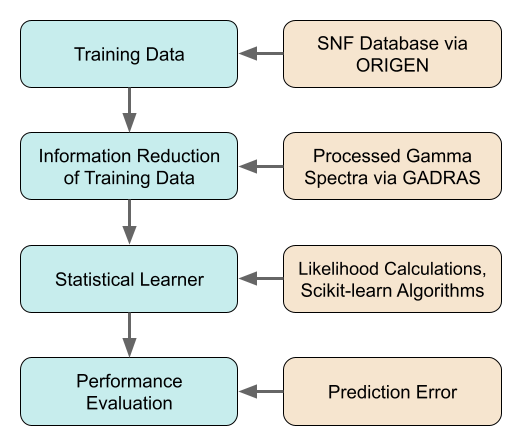
\includegraphics[width=0.7\linewidth]{./chapters/exp2/methodology2.png}
  \caption[Experimental methodology in Chapter \ref{ch:exp2}]
          {Flowchart of the experimental methodology and the way each step is 
           being implemented.}
  \label{fig:method2}
\end{figure}

The full description of the simulations and training labels can be found in
Section \ref{sec:training1}.  Section \ref{sec:training2} provides the updates
on the features used in the training set.  This results in a set of \gls{SNF}
observations with the same known reactor operation parameters, i.e., labels
that are to be predicted, but new nuclide features. 

Next, the information reduction step is covered in Section
\ref{sec:inforeduc2}.  Here, computational gamma spectra are created via the
\gls{GADRAS} tool; six detectors with decreasing energy resolution were chosen.
The approach for processing the spectra from these detectors is outlined here
as well. 

The increasingly less-precise training data sets are input to a statistical
learner for the next step: training models.  These use the features (from
processed spectra) and labels (reactor parameters/simulation inputs) in the
training data sets to formulate a model.  This is introduced in Section
\ref{sec:statmodel1}, and the updates for this experiment are in Section
\ref{sec:statmodel2}. 

Lastly, the algorithms must be evaluated for their prediction performance when
given test samples (i.e., a new \gls{SNF} measurement that has no labels
according the to algorithm).  This follows much of what was introduced in
Section \ref{sec:eval1}, and the updates to the approach is shown in Section
\ref{sec:eval2}. 

\section{Training Data Simulation}
\label{sec:training2}
\begin{figure}[H]
  \centering
  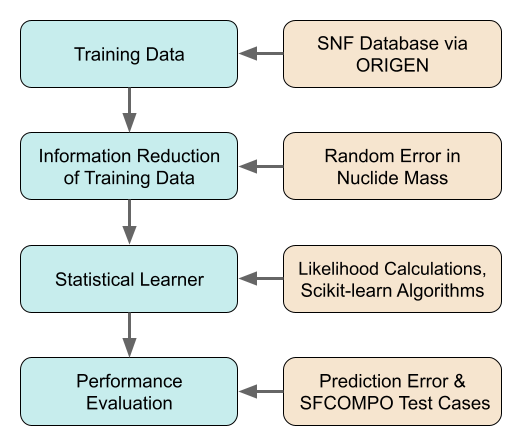
\includegraphics[width=0.7\linewidth]{./chapters/exp1/methodology1.png}
  \caption{First portion of the flowchart from Figure \ref{fig:method} being 
           described in this section.}
\end{figure}

Of interest to an entity trying to create a weapon is partially irradiated fuel
if they have plutonium separations capabilities or any radioactive substance in
the case of a dirty bomb. Thus, this work focuses on \gls{SNF} from commercial
power reactors. Ideally, a large enough database of \gls{SNF} nuclide assays
would be able to be used for this work. Since that does not exist, the 
database will be simulated via \gls{ORIGEN-ARP} \cite{origen, origenarp}.  

\subsection{Simulation Fidelity}
\label{sec:fidelity}

Nuclear fuel cycle studies involve tracking the material flow of nuclear fuel.
This can be anywhere from mining to waste management, or focus on a process
step in between. Fuel cycle studies are not necessarily nuclear-specific. For
example, they can be used to evaluate economic predictions, environmental
impact, transportation planning, etc.  In order to draw conclusions from these
studies, it is common to use a nuclear fuel cycle simulator that tracks the
quantities of interest. These allow the comparison of different fuel types,
reactor technologies, material processing steps, etc. 

There are simplifications researchers need to make in order to experiment in a
controlled way. Fuel cycle simulators, built for a specific needs, must remove
complicating factors that are less relevant to the study.  For example, one
tool might be suited well to large-scale systems analysis with little nuclear
physics included in the models, and another might focus on detailed isotopics
within a system to track plutonium.

Because a large portion of a nuclear forensics investigation relies on
measuring isotopics, this work used \gls{ORIGEN} \cite{origen}, which is a part
of the \gls{SCALE} 6.2 modeling and simulation suite of computational tools
developed for nuclear design and safety \cite{scale}. \gls{ORIGEN} was chosen
for its physically detailed models of activation, depletion, and decay.
Specifically, the ARP module of the code was used: \gls{ORIGEN-ARP}
\cite{origenarp}.

\gls{ORIGEN} calculates time-dependent nuclide concentrations (or quantities
derived from these) that result from activation and depletion calculations. The
physics (i.e., neutron transport and decay) calculations are carried out in
other \gls{SCALE} modules that solve the depletion equations.  This generates
libraries for \gls{ORIGEN} that include the probabilities of reaction (i.e.,
cross sections) for the system.

To obtain an \gls{SNF} recipe from a reactor simulation, \gls{ORIGEN} uses the
desired input power generation with the cross section library to calculate a
flux, the resulting depletion, and the end composition (i.e., isotopic recipes
or nuclide vectors).  Another output is decay; the composition is computed
using decay equations with nuclear data \cite{endf}. These compositions provide
source terms for other calculations, such as decay emission spectra from
neutrons, alpha particles, beta particles, and gamma rays. Other derived
quantities like activity, decay heat, or radiological hazard factors are also
an option.

\gls{ORIGEN-ARP} allows users to access a wider range of simulations by
interpolating between the pre-calculated libraries instead of creating new
libraries.  It is known to be validated for \gls{LWR} \gls{SNF}
\cite{lwr_valid}. Additionally, recycled \gls{SNF} in the form of mixed oxide
fuel has been benchmarked for the relevant reactors \cite{mox_valid}.  Through
\gls{ORIGEN}, given an initial material composition, some reactor operation
parameters, and a reactor type, one can quickly perform many different nuclear
reactor simulations and obtain \gls{SNF} recipes.

\todo[inline]{This section needs more information about ORIGEN-ARP validation
and maybe some nuclides that are known to perform poorly from ARP sims. Can
show a generic example from one of my sources, and or an example of trying to
match an ORIGEN-ARP simulation to an SFCOMPO entry. It is important to inform
that this training set as ground truth is not perfect truth, for some nuclides
more than others. The goal is to explain the ARP validation without getting
too deep.  This tool was necessary for the 500k training set. The prediction
performance will be impacted by the poorly simulated nucs, so it may be
worthwhile to note which ones have consistently large sim errors (unless this
involves getting too deep). P.S. did you mention homogenized core above?}

\subsection{Training Set Labels}
\label{sec:snflbls}

\begin{table}[!htb]
  \centering
  \begin{subtable}{\linewidth}
    \centering
    
\includegraphics[width=0.5\linewidth]{./chapters/exp1/trainset4_Orxtrs.png}
    \caption{\gls{ORIGEN} designations for reactor technologies and fuel assembly design.}
    \label{tbl:rxtrtype}
    \vspace*{5mm}
  \end{subtable}
  \begin{subtable}{\linewidth}
    \centering
    
\includegraphics[width=0.75\linewidth]{./chapters/exp1/trainset4_inputs.png}
    \caption{Simulation parameters for \gls{ORIGEN} input files.}
    \label{tbl:rxtrparam}
  \end{subtable}%
  \caption{Training set database design using the \gls{SFCOMPO} database as guidance. \cite{sfcompo}}
  \label{tbl:train}
\end{table}

The design of the training set is dependent on a number of factors.  First, it
must have a sufficient number of burnup sets and time since irradiation steps
to provide robust prediction. This is decided upon by maximizing the steps for
both parameters, while balancing the computational limitations of a large
training set. Through previous experience, an approximate limit would be around
$1e6$ database entries for the specific calculations in this work and employing
reasonable computational limitations.

Secondly, the training set must represent what exists in the real world. This
was accomplished by studying the spread of parameters in the \gls{SFCOMPO}
database \cite{sfcompo}.  To ensure this, a variety of reactor types and
assembly designs were included, listed in Table \ref{tbl:rxtrtype}. Table
\ref{tbl:rxtrparam} lists the rest of the simulation inputs. These include not
only the labels of prediction interest, \gls{U235} enrichment, burnup, and time
since irradiation, but also other important simulation input parameters such as
the reactor power density and the moderator density.  (Water is both the
moderator and coolant in all simulated reactor types.)

\begin{figure}[!hbt]
  \makebox[\textwidth][c]{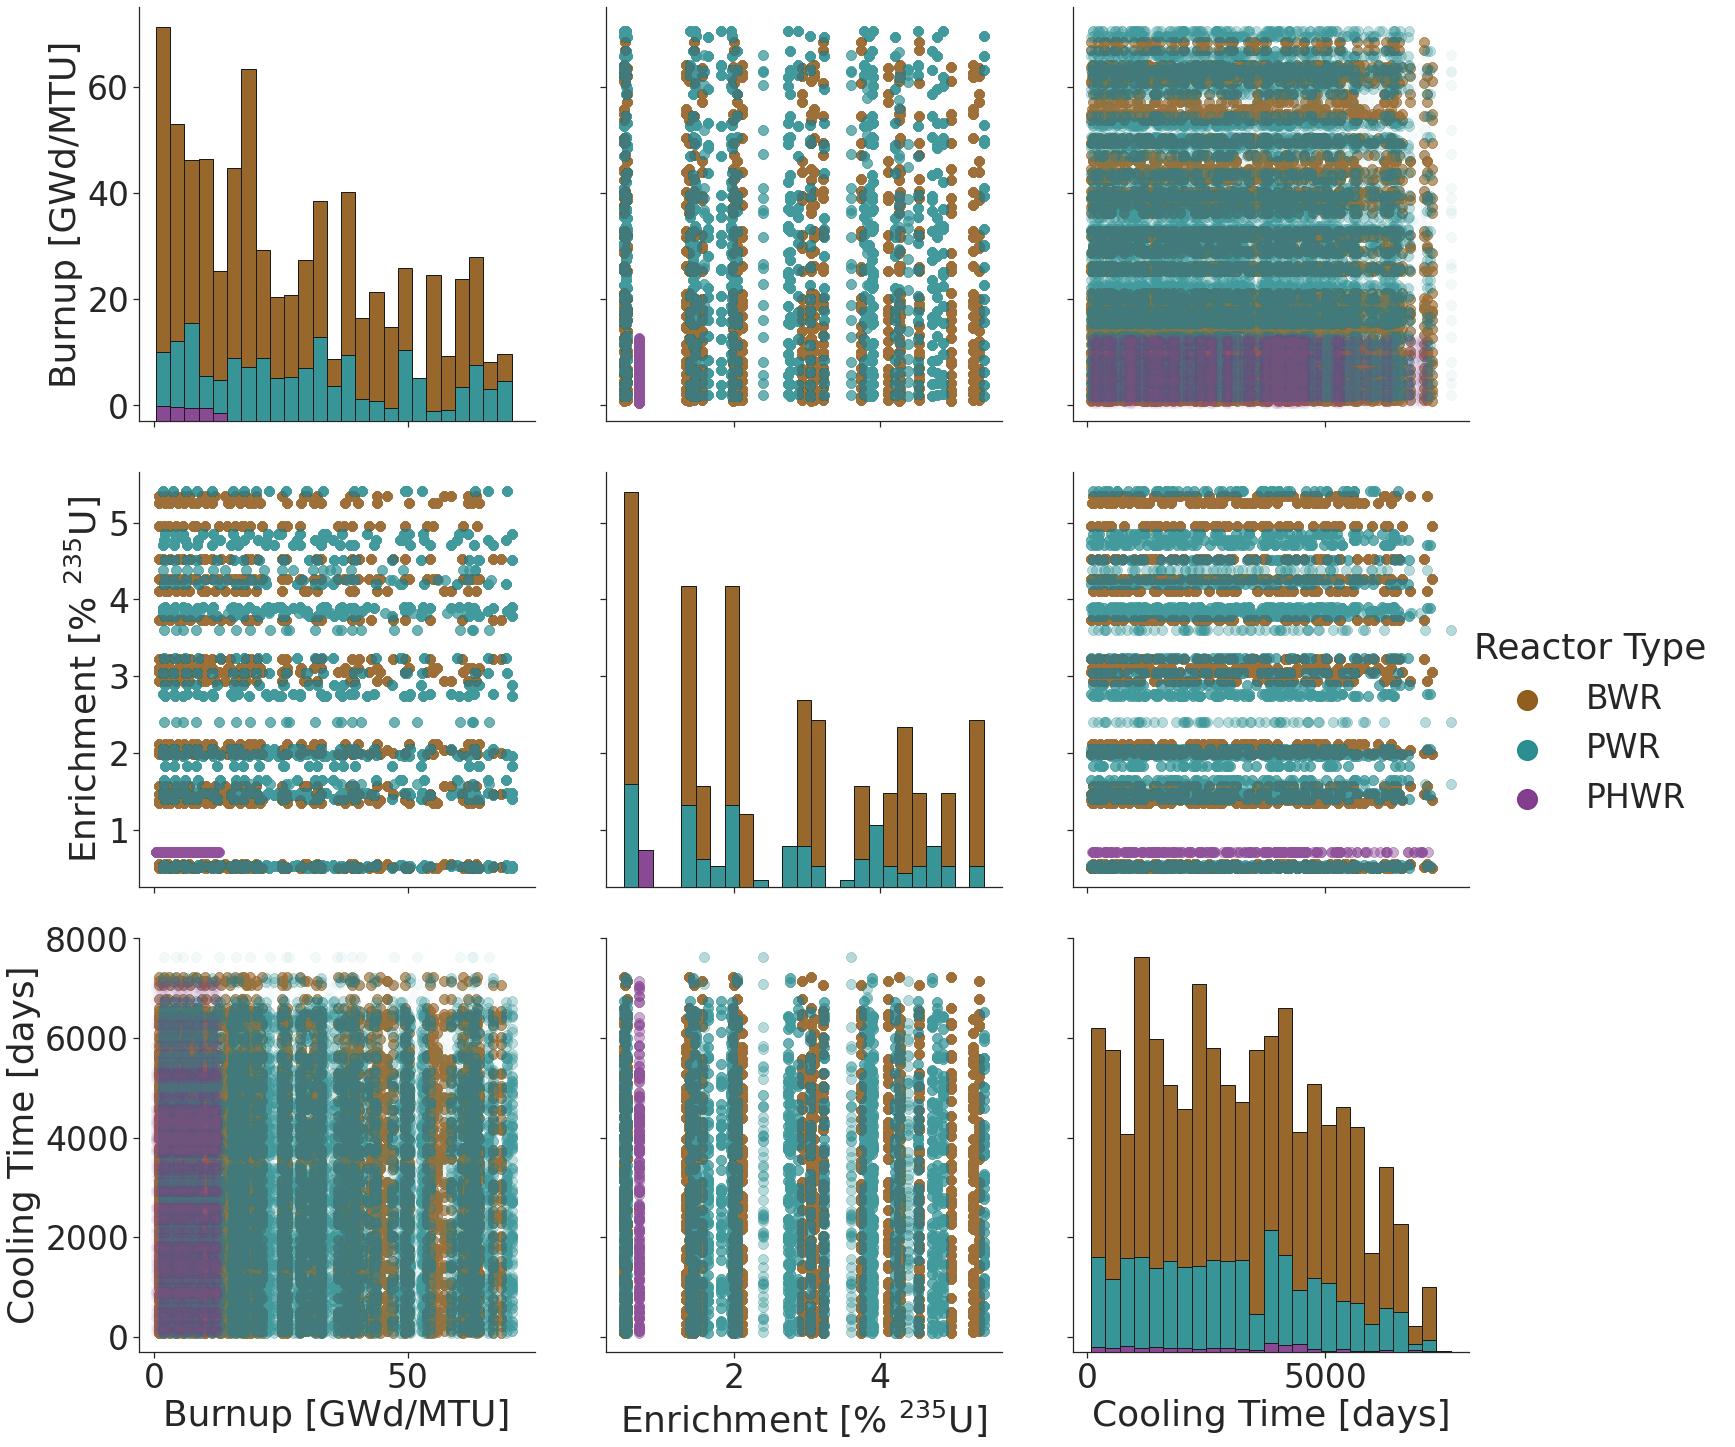
\includegraphics[width=\linewidth]{./chapters/exp1/histogram_scatter_trainset_viz.png}}
  \caption{A combination of histograms and scatter plots to visualize the 
           distribution of prediction labels in the training set.}
  \label{fig:trainhist}
  \todo[inline]{fix the histogram figure, this is a placeholder}
\end{figure}

The third factor influencing database design is ensuring ideal \gls{ML}
algorithm performance.  As mentioned in Section \ref{sec:errs}, many algorithms
are developed with the assumption that the training set will be
\acrfull{i.i.d.}.  This is important so that the model does not overvalue or
overfit a certain area in the training space. With the training set design,
there are predetermined values for enrichment, burnup, and time since
irradiation.  While there are $21-28$ burnup steps (depending on the reactor
type) and 61 cooling time steps, there are only 6 values for enrichment. This
creates the risk that the algorithm will end up being unable to generalize
outside of those discrete values. Therefore, the burnup steps and time steps
are perturbed randomly in a range that is $\pm10\%$ and $\pm30\%$ from the
originally defined values, respectively.  The enrichment also gets perturbed by
$\pm10\%$, and not more because the cross-section libraries in \gls{ORIGEN-ARP}
are pre-calculated for those enrichment values, so deviating too far from them
would result in inaccurate \gls{SNF} simulations. The power densities and
moderator densities were kept at the values defined in Table
\ref{tbl:rxtrparam}.  The resulting training set is $450240$ (or $4.5e5$)
entries.  Figure \ref{fig:trainhist} visualizes the somewhat even distribution
of the burnup and cooling time parameters, and shows the lack of even
distribution of the enrichment parameter through a combination of scatter plots
and histograms.  Note that there are many more \gls{BWR}s present in the
histograms because of the multiple moderator densities simulated (see Table
\ref{tbl:rxtrparam})

\subsection{Training Set Features}
\label{sec:snffeats}

The other design decision regarding the training set is related to
which nuclides to track, i.e., the features.  For this experiment, nuclide
masses are necessary, and the most common measurements in \gls{SFCOMPO} guide
the list of nuclides tracked.  

The set of training features of 29 nuclide masses listed in Table
\ref{tbl:nucmass} was designed with the following reasons in mind.  First, the
units in mass is to represent the scenario of "perfect knowledge", where a full
assay is done via mass spectrometry techniques.  Second, this is to have the
training set units convertable to those present in the external, real-world
test set: the \gls{SFCOMPO} database.  The \gls{ORIGEN} simulations output the
nuclide masses in $grams$, and they are converted to the units of
\textit{milligrams per gram of initial uranium}, $mg/gU_i$, when the models are
externally tested against \gls{SFCOMPO}. Lastly, the 29 nuclides chosen were
based on the presence of measurements in \gls{SFCOMPO}, where these were
present in at least 100 of the samples in the database.  The external test set
is described in more detail in Section \ref{sec:sfcompo}.

\begin{table}[!htb]
  \centering
  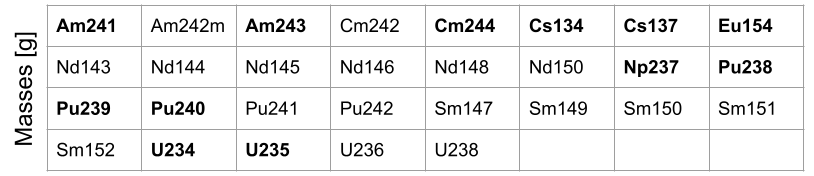
\includegraphics[width=\linewidth]{./chapters/exp1/nucmass_feats.png}
  \caption{Set of features saved for the first experiment, nuclide masses 
           measured in $grams$. The bold nuclide masses overlap with the 
           nuclides in \ref{tbl:nucacts}.}
  \label{tbl:nucmass}
\end{table}



\section{Information Reduction}
\label{sec:inforeduc2}

\begin{figure}[H]
  \centering
  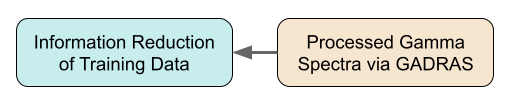
\includegraphics[width=0.7\linewidth]{./chapters/exp2/methodology2_2.png}
  \caption[Second portion of the flowchart from Figure \ref{fig:method2}]
          {Second portion of the flowchart from Figure \ref{fig:method2} being 
           described in this section.}
\end{figure}

The overall goal of this project is to determine how much information to what
quality is needed to train a  \gls{ML} model that can provide \gls{SNF}
attribution by correctly predicting the reactor type, burnup, \gls{U235}
enrichment, and time since irradiation.  In this section, the information
quality is treated as the energy resolution of gamma spectra from several
detectors.  This is because field-deployable detectors are of interest.

This process is outlined here for the second experiment, in which a gamma
spectrum is computed for each sample in the database from the nuclide
activities in Section \ref{sec:training2}.  The \gls{GADRAS} code \cite{gadras}
developed at Sandia National Laboratories will provide computational gamma
spectra. There are four steps to this process: choosing radionuclides,
inputting the radionuclide activities into a \gls{DRF} to compute gamma
spectra, processing the gamma spectra into a smaller feature set, and applying
a statistical counting error to those features.

\noindent \textbf{Step 1: Choosing Radionuclides}

The first step of is covered in Section \ref{sec:training2}.  

\noindent \textbf{Step 2: Computational Gamma Detection}

The second step is obtaining a gamma spectrum for every \gls{SNF} entry in the
database; this is done using \gls{GADRAS}. The \gls{GADRAS} tool includes many
capabilities related to radiation detection and spectra analysis; its
predominant use is related to the simulation of the detection of gamma rays and
neutrons from user-defined sources and detector configurations.  A combined
first principles and empirical modeling approach based on interaction cross
sections and radiation scattering inform the \glspl{DRF} code to calculate
typical gamma detector spectrum features, e.g., photopeaks and the Compton
continuum.  Although new detectors can be created and calibrated within the
software, this work employs the use of pre-calibrated detectors.  Thus, given a
source, which is a list of radionuclides and their activities in this case,
\gls{GADRAS} applies a \gls{DRF} from a given detector configuration to the
gamma energy lines from these radionuclides and models the spectrum.
\cite{gadras} 

The nuclide activity data requires some processing to be used in this way.  The
activities that come from the \gls{ORIGEN} simulations are based on there being
$1\:MT$ of initial uranium-based fuel. Not only is this quantity an unlikely
amount to be smuggled, it would overwhelm a detector at the calibrated
source-detector distances in \gls{GADRAS}.  Therefore, the material (and
resulting nuclide activities) are scaled to be $1\:g$ of \gls{SNF}.

For the \gls{GADRAS} calculations, the primary input is a nuclide activity
vector as the source, and the output is an array of energy bins (measured in
$keV$) and the counts per energy bin as the spectrum.  The sources are provided
without any background; this is because any spectrum would undergo background
subtraction before further analysis. Additionally, the nuclides are pre-decayed
in \gls{ORIGEN} to correspond to various cooling times, but a source age must
be provided to \gls{GADRAS} as a non-zero value (otherwise, important decay
transitions are missed). Various source times ($10\:sec$, $30\:sec$, $1\:min$,
$5\:min$, $10\:min$, $20\:min$, $30\:min$, $1\:hr$, $2\:hr$) were tested for
two samples, and both a qualitative visual analysis of the major photopeaks
plus a study of the total counts leveling off was used to choose a nonzero age
for the material.  At a source age of $20\:minutes$, the expected peaks are
visible and the total counts had reached a value similar to the longer ages
tested.

The other input information is related to the detector configuration.
User-chosen variables are the source-detector distance $[cm]$, height of
source-detector setup from nearest surface $[cm]$, the live time $[s]$, and the
number of channels for the detector. The detector configuration file in
\gls{GADRAS} contains much more information, however.  In it, there are a
number of parameters from calibration results, detector geometry, information
about scattering, and shielding information (shielding is not considered in
this work).

\begin{table}[!htb]
  \centering
  \begin{tabular}{@{}lcllll@{}}
  \toprule
    \textbf{Detector} &
    \textbf{\begin{tabular}[c]{@{}c@{}}\% FWHM \\ @ 661 keV\end{tabular}} &
    \textbf{\begin{tabular}[c]{@{}l@{}}Distance \\ (cm)\end{tabular}} &
    \textbf{\begin{tabular}[c]{@{}l@{}}Height \\ (cm)\end{tabular}} &
    \textbf{\begin{tabular}[c]{@{}l@{}}Live Time\\ (s)\end{tabular}} &
    \textbf{\begin{tabular}[c]{@{}l@{}}Num \\ Channels\end{tabular}} \\ \midrule
    In-Lab HPGe           & 0.21 & 100.0 & 84.0  & 600  & 8192 \\
    Portable HPGe         & 0.29 & 100.0 & 100.0 & 600  & 8192 \\
    CZT                   & 1.20 & 100.0 & 100.0 & 600  & 1024 \\
    SrI\textsubscript{2}  & 2.94 & 100.0 & 100.0 & 600  & 1024 \\
    LaBr\textsubscript{3} & 3.63 & 213.0 & 84.5  & 2400 & 1024 \\
    NaI                   & 7.74 & 213.0 & 85.4  & 2400 & 1024 \\ \bottomrule
  \end{tabular}
  \caption[Details of detector setups]
          {Select details of 6 detector setups used to obtain gamma 
           spectra-based training databases.}
  \label{tbl:detsetups}
\end{table}

Training databases were created for the six detectors outlined in Table
\ref{tbl:detsetups}. They were chosen to compare the highest energy resolution
detector, a lab-based \gls{HPGe}, against the rest, in order of decreasing
energy resolution: portable \gls{HPGe}, \gls{CZT}, \gls{SrI2}, \gls{LaBr3}, and
\gls{NaI} detectors. This is displayed in the table by including the \gls{FWHM}
of the $661\:keV$ peak for ${}^{137}\text{Cs}$. \Gls{GADRAS} is used to create
a spectrum for every \gls{SNF} entry in the 32 nuclide activity training
database using these six detector configurations.  At this point, there are six
versions of the original database, one for each detector.  The database entries
are each a full gamma spectrum of a given \gls{SNF} sample for the detector
setup in that training set. 

\noindent \textbf{Step 3: Processing Gamma Spectra}

The third step covers the processing of the gamma spectrum generated for each
\gls{SNF} entry into a training set.  It is not computationally prudent to use
full gamma spectra for training and testing, since the spectra returned have
1024 or 8192 bins, and machine learning algorithms are not designed to handle
thousands of features.  Thus, these spectra are processed into fewer features; 
this is outlined as follows.

There is much ongoing work on the topic of attributing \gls{SNF} with gamma
detection using targeted or advanced measurement techniques \cite{snf_gamma,
compton_supp, bwr_high-res_gamma, pwr_bwr_gamma} and using innovative spectra
evaluation and radioisotope identification methods \cite{riid_09,
rapid_riid_18, sull_gen_07, sull_valid_15, sull_auto_17, sull_unc_17}.  \todo{update citations} Since
this is a topic of active research and the approaches are heavily
detector-dependent, a simple processing approach is developed here.  Since all
entries in a given training set are background-subtracted spectra using the
same detector setup and calibration for the same measurement duration, each
photopeak can be directly compared to other photopeaks in the training set.
This is accomplished by comparing them via an area under the curve: placing an
energy window on a peak, and summing the counts of the bins within that energy
window. 

There are two main design choices here: the width of the energy windows and the
number of energy windows to include. First, the energy window width is a value
that is fixed for each detector prior to processing.  The different energy
window widths are listed in Table \ref{tbl:enwindows}.  They are chosen
manually; the spectra were plotted and different values were tested and
visually analyzed to be sure the windows were encompassing the peaks. This was
preferable to some linear function based on the detector energy resolution
because, e.g., the \gls{LaBr3} and \gls{NaI} detectors have the same
human-chosen window but the energy resolutions are different (see Table
\ref{tbl:detsetups}). 

\begin{table}[!htb]
  \centering
  \begin{tabular}{@{}lcm{0.7in}m{0.7in}m{0.7in}@{}}
    \toprule
    \multirow{2}{*}{\textbf{Detector}} &
    \multirow{2}{*}{\textbf{\begin{tabular}[c]{@{}l@{}}Energy Window\\ Size {[keV]}\end{tabular}}} &
    \multicolumn{3}{c}{\textbf{\# of Energy Windows}} \\ \cmidrule(l){3-5}
                     &    & Auto & Short & Long \\
    \toprule
    In-Lab HPGe      & 2  & 206  & 42    & 151  \\
    Portable HPGe    & 3  & 120  & 42    & 151  \\
    CZT              & 8  & 30   & 42    & 151  \\
    $\text{SrI}_2$   & 10 & 17   & 42    & 151  \\
    $\text{LaBr}_3$  & 12 & 19   & 42    & 151  \\
    NaI              & 12 & 9    & 42    & 151  \\ 
    \bottomrule
  \end{tabular}
  \caption[Energy window sizes and list lengths for processing gamma spectra]
          {Energy window sizes and list lengths for 6 detector setups used to 
           process the gamma spectra-based training databases.}
  \label{tbl:enwindows}
\end{table}

The second design decision is the number of energy windows to include.  Table
\ref{tbl:enwindows} lists three energy window list length columns,
\textit{Auto}, \textit{Short}, and \textit{Long}. These correspond to different
processed training sets that have a different number of energy windows
included.  There are two approaches taken: a nuclear physics-based method that
generates an energy window list based on the gamma energies expected to be
detected (short and long), and an automatic peak search of a manually chosen
gamma spectrum in the full gamma spectra training database (auto). 

The first energy window list method provides the short and long lists in Table
\ref{tbl:enwindows}; the length of these lists are the same for all detectors
because they are based on the gamma energies most likely to be detected, which
is independent of the detector quality. To obtain these lists, the expected
number of decays of each gamma energy is calculated based on the activities of
the 32 tracked nuclides using the Python for Nuclear Engineering toolkit
\cite{pyne} from a reference sample in the training set.  This reference sample
emerged as the sample of choice because it contains the superset of gamma
energies of all tested samples, of which there were nine (three for each
reactor type).

After the expected number of decays for each gamma energy for all 32 nuclides
are calculated, an arbitrary minimum number of decays is selected to filter out
the gamma energies that are unlikely to produce counts high enough to be
detected. The first arbitrary minimum number of decays is set at $5 \times
10^8$ decays, and the long list of 151 gamma energies that remain above this
cutoff is created.  A list of length 151 is likely to contain many features
that do not contribute discrimination to the models, and thus they may add
noise to the training set, so a shorter list is needed.  So, a higher arbitrary
minimum of $5 \times 10^{10}$ decays is chosen; this threshold creates the
short list of 42 gamma energies. 

The short and long lists of gamma energies correspond to the nuclides in Table
\ref{tbl:enlistnucs}. The 12 nuclides listed come from the long list, and the
subset of seven bold nuclides come from the short list.  To determine a "full
knowledge" scenario for the detector-based training sets, two training sets are
also created with the 7- and 12-nuclide activity lists.  It should be noted
that several (three for each reactor type) training set entries were selected
based on sampling evenly throughout the training set parameters, with the
intention that there would be a set of gamma energies comprised from multiple
entries. However, one sample emerged as a superset of the others. This sample
is thus chosen for the second method, discussed next.

\begin{table}[!htb]
  \centering
  \begin{tabular}{@{}|l|l|l|@{}}
    \hline
    \allbold{${}^{241}\text{Am}$} & \allbold{${}^{243}\text{Am}$} & ${}^{243}\text{Cm}$           \\ \hline
    ${}^{244}\text{Cm}$           & ${}^{245}\text{Cm}$           & \allbold{${}^{134}\text{Cs}$} \\ \hline
    \allbold{${}^{137}\text{Cs}$} & ${}^{152}\text{Eu}$           & \allbold{${}^{154}\text{Eu}$} \\ \hline
    \allbold{${}^{85}\text{Kr}$}  & ${}^{238}\text{Pu}$           & \allbold{${}^{125}\text{Sb}$} \\ \hline
  \end{tabular}
  \caption[Nuclides that are represented by the short and long energy windows 
           lists]
          {Nuclides that are represented by the gamma energy lines in the 
           energy lists. The entire set of 12 nuclides belongs to the long 
           list, and the 7 bold nuclides belong to the short list.}
  \label{tbl:enlistnucs}
\end{table}

The column denoted as \textit{Auto} in Table \ref{tbl:enwindows} is obtained by
a physics-free approach. It is based on a peak search of a spectrum in the full
gamma spectra training database. The previously mentioned sample is selected
for all six detectors, and a peak searching algorithm implemented in python
using the SciPy toolkit \cite{scipy} is applied. Using the peak search on the
six different spectra for the same sample, the resulting number of energy
windows for each detector is in Table \ref{tbl:enwindows}.  

%this is idx 66796
\begin{figure}[!htb]
  \makebox[\textwidth][c]{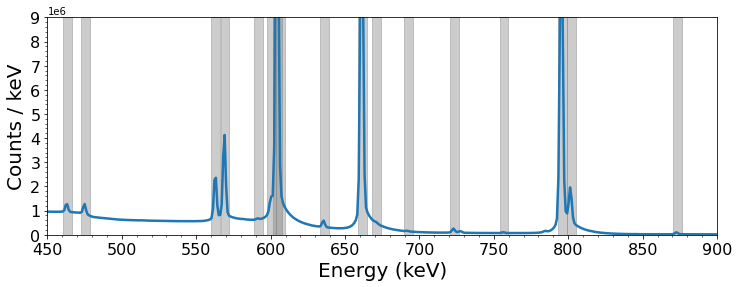
\includegraphics[width=\linewidth]{./chapters/exp2/energy_window_example.png}}
  \caption[Portion of gamma spectrum with windows, which shows summation regions 
           for spectra processing]
          {Slice of an example gamma spectrum in one of the training databases
           showing the windows over the gamma energy peaks. This is the portable
           \acrshort{HPGe} with the auto energy window list and the reference 
           sample's spectrum.}
  \label{fig:enwindows}
\end{figure}

After the three energy window lists are created, the full gamma spectra
database of a given detector are processed into three training sets, one for
each list.  Next, as previously mentioned, the energy window width for each
detector is used to sum the binned counts for each energy window list entry.
this is visualized in Figure \ref{fig:enwindows}, where a portion of a portable
\gls{HPGe} spectrum is shown with the $\pm3\:keV$ windows from the auto energy
window list.  Three training sets are created for each detector, resulting in
18 detector-based processed gamma spectra training sets.

\noindent \textbf{Step 4: Apply Statistical Counting Error}

Lastly, the fourth step involves the inclusion of the counting error for the
summed energy windows. This is quite simple mathematically speaking, as
statistical counting error of $n$ counts is $\sqrt{n}$.  As in Section
\ref{sec:inforeduc1}, this error gets applied in the same way for the
scikit-learn algorithms, where the uniform error is applied randomly within the
range $[x_i - \sqrt{x_i}, x_i + \sqrt{x_i}]$ for each summed energy window
$x_i$. For the \gls{MLL} calculations, Equation \ref{eq:mllunc} is used, where
$\sigma_{i} = \sqrt{x_i}$.  

In summary, there are four steps taken to arrive at training databases based on
gamma spectra from six chosen detectors. Unlike the simple increase in training
set error applied in Chapter \ref{ch:exp1}, each step of the process adds an
additional layer of reduced information quality, which are listed here:
\begin{enumerate}
  \item The list of nuclides is limited to manually chosen radionuclides.
  \item Instead of "perfect" radionuclide activity knowledge, they are being 
        measured by a gamma detector.
  \item The processing of the gamma spectra can be highly variable.
  \item The $\sqrt{n}$ error of counts-based detection is included. 
\end{enumerate}



\section{Statistical Learning Implementation}
\label{sec:statmodel2}

\begin{figure}[H]
  \centering
  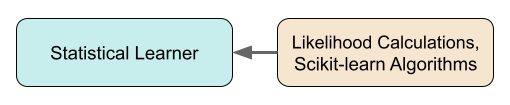
\includegraphics[width=0.7\linewidth]{./chapters/exp2/methodology2_3.png}
  \caption[Third portion of the flowchart from Figure \ref{fig:method2}]
          {Third portion of the flowchart from Figure \ref{fig:method2} being 
           described in this section.}
\end{figure}

The chosen algorithms (\textit{k}-nearest neighbors, decision trees, and
\gls{MLL} calculations) are introduced in Section \ref{sec:algs} and their
implementation details are in Section \ref{sec:statmodel1}.  This section will
therefore only cover the implementation differences from the previous work.
The \gls{MLL} calculations are implemented identically to Chapter
\ref{ch:exp1}.  However, the scikit-learn algorithms in this experiment did
undergo a new round of hyperparameter optimization.

The full list of 22 training sets that undergo training and prediction are as
follows: 
\begin{itemize}
  \item 1 set of nuclide masses (29 nuclide masses from Chapter \ref{ch:exp1})
  \item 3 sets of nuclide activities
    \begin{itemize}
      \item 32 nuclide activities (full knowledge scenario for all nuclides, 
            whether or not they are present in a quantity able to be detected)
      \item 12 nuclide activities (full knowledge for long energy windows list)
      \item 7 nuclide activities (full knowledge for short energy windows list)
    \end{itemize}
  \item 18 detector-based processed spectra sets
    \begin{itemize}
      \item Auto energy windows lists applied to six detectors (lab-based 
            \gls{HPGe}, portable \gls{HPGe}, \gls{CZT}, \gls{SrI2}, \gls{LaBr3}, 
            \gls{NaI})
      \item Short energy windows lists applied to six detectors above
      \item Long energy windows lists applied to six detectors above
    \end{itemize}
\end{itemize}

\begin{table}[!htb]
  \centering
  \begin{tabular}{@{}llcll@{}}
    \toprule
    \textbf{\begin{tabular}[c]{@{}l@{}}Training Set\\ Description\end{tabular}} &
    \textbf{\begin{tabular}[c]{@{}l@{}}Prediction\\ Parameter\end{tabular}} &
    \textbf{\begin{tabular}[c]{@{}l@{}}\textit{k} \\ (N neighbors)\end{tabular}} &
    \textbf{\begin{tabular}[c]{@{}l@{}}Max \\ Depth\end{tabular}} &
    \textbf{\begin{tabular}[c]{@{}l@{}}Max \\ Features\end{tabular}} \\ 
    \toprule
    \multirow{4}{*}{\begin{tabular}[c]
    {@{}l@{}}29 \\ Nuclide\\ Masses\end{tabular}}          & Reactor Type & 4 & 56 & 29          \\
                                                           & Burnup       & 1 & 77 & 29          \\
                                                           & Enrichment   & 1 & 73 & 29          \\
                                                           & Cooling Time & 2 & 45 & 29          \\ 
                                                           \hline
    \multirow{4}{*}{\begin{tabular}[c]
    {@{}l@{}}32\\ Nuclide\\ Activities\end{tabular}}       & Reactor Type & 1 & 41 & 32          \\
                                                           & Burnup       & 1 & 49 & 32          \\
                                                           & Enrichment   & 1 & 67 & 32          \\
                                                           & Cooling Time & 7 & 56 & 32          \\
                                                           \hline
    \multirow{4}{*}{\begin{tabular}[c]
    {@{}l@{}}7 or 12\\ Nuclide \\ Activities\end{tabular}} & Reactor Type & 1 & 67 & 7 or 12     \\
                                                           & Burnup       & 1 & 78 & 7 or 12     \\
                                                           & Enrichment   & 1 & 60 & 7 or 12     \\
                                                           & Cooling Time & 4 & 68 & 7 or 12     \\
                                                           \hline
    \multirow{4}{*}{\begin{tabular}[c]
    {@{}l@{}}Energy \\ Windows:\\ Short\end{tabular}}      & Reactor Type & 1 & 62 & 42          \\
                                                           & Burnup       & 1 & 62 & 42          \\
                                                           & Enrichment   & 4 & 64 & 42          \\
                                                           & Cooling Time & 2 & 54 & 42          \\
                                                           \hline
    \multirow{4}{*}{\begin{tabular}[c]
    {@{}l@{}}Energy \\ Windows:\\ Long\end{tabular}}       & Reactor Type & 4 & 62 & 151         \\
                                                           & Burnup       & 1 & 51 & 151         \\
                                                           & Enrichment   & 5 & 73 & 151         \\
                                                           & Cooling Time & 2 & 64 & 151         \\
                                                           \hline
    \multirow{4}{*}{\begin{tabular}[c]
    {@{}l@{}}Energy \\ Windows:\\ Auto\end{tabular}}       & Reactor Type & 2 & 61 & None or 150 \\
                                                           & Burnup       & 1 & 52 & None or 150 \\
                                                           & Enrichment   & 4 & 67 & None or 150 \\
                                                           & Cooling Time & 2 & 58 & None or 150 \\ 
    \bottomrule 
  \end{tabular}
  \caption[Optimized algorithm hyperparameters for all training sets in second 
           experiment]
          {Optimized algorithm hyperparameters; the energy lists took all 
           detectors into account.}
  \label{tbl:exp2hypparam}
\end{table}

Table \ref{tbl:exp2hypparam} lists the hyperparameter optimization results for
the 22 training sets. Because the 29 nuclide mass training set is included in
this chapter for comparison, its optimization results are also listed here.
The number of features for decision trees are not limited because the test runs
for optimization provided highly variable results. The only case where this is
not true is with the auto energy windows list for the lab-based \gls{HPGe} with
a length of 206; the maximum features for this one case are limited to 150.
Instead, optimization was carried out only on the maximum depth for decision
trees with keeping the full length of features.  This is an area that could
undergo deeper exploration than what occurs in this work, since the training
sets with large feature sets can become overfit.

The optimization took place in two rounds, where the first round had a coarser
grid of \textit{k} for \textit{k}-nearest neighbors and maximum depth for
decision trees and the second round had a finer grid of parameters. The 7 \& 12
nuclide activity training sets were optimized separately but contain averages
of the two results for the maximum depth, and the higher value of \textit{k}
when the two did not match. The \textit{k} and maximum depths were averaged
across all six detectors for each energy window list length (short, long, and
auto).  There were fairly consistent results from the short and long lists, but
the variable length of the auto-generated energy windows lists (in Table
\ref{tbl:enwindows}) gave a wider range of ideal hyperparameters.



\section{Performance Evaluation}
\label{sec:eval2}

\begin{figure}[H]
  \centering
  
\includegraphics[width=0.7\linewidth]{./chapters/exp1/methodology1_4.png}
  \caption[Fourth portion of the flowchart from Figure \ref{fig:method1}]
          {Fourth portion of the flowchart from Figure \ref{fig:method1} being 
           described in this section.}
\end{figure}

As previously introduced in Section \ref{sec:testerr}, the prediction
performance is measured by evaluating the accuracy of the reactor type
classification or the error of the regression cases (burnup, \gls{U235}
enrichment, cooling time).  These performance metrics for all four prediction
types are compared across the three algorithms used: \textit{k}-nearest
neighbors (denoted in plots as \textit{kNN}), decision trees (denoted in plots
as \textit{Dec Tree} or \textit{DTree}), and \gls{MLL} calculations.  

\subsection{Random Error Impacts on Prediction}
\label{sec:randerr}

To judge the degradation of predictions of the algorithms with increasing
nuclide mass measurement error (i.e., reduced information quality, detailed in
Section \ref{sec:inforeduc1}), several plots are made with the introduced error
on the \textit{x}-axis and a prediction performance metric on the
\textit{y}-axis.  The \textit{y}-axis is always oriented so that lower is
poorer performance and higher is better performance. This is why Figures
\ref{fig:randburn}--\ref{fig:randcool} present a negative error on the
\textit{y}-axis. Additionally, the data points on all the plots have a small
$\Delta x$ to show error bars that are otherwise impossible to see.

In all of the results in this section, the statistics being reported is on all
$4.5 \times 10^5$ entries in the training set.

\subsubsection{Reactor Type Classification}
\label{sec:randerrA}

Figure \ref{fig:randrxtr} shows the balanced accuracy of reactor type
classification, where a score of $1$ is perfect prediction and a score of $0$
is random classification. The error bars reflect a 99\% confidence interval.
While the two scikit-learn algorithms follow a very similar path of decreased
accuracy as the error increases, the \gls{MLL} calculation approach appears to
be more robust to the nuclide mass measurement error.  Another interesting
result is that the \gls{MLL} calculation performs slightly worse for low
errors. If the expected measurement errors of nuclide masses in a training
database or in a test sample can be guaranteed to be better than ~2\%, the
\gls{MLL} calculation is no longer the obvious preferred choice for reactor
type prediction.

\begin{figure}[!htb]
  \centering
  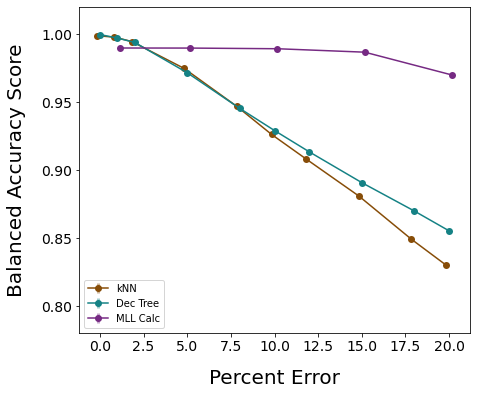
\includegraphics[width=0.5\textwidth]{./chapters/exp1/randerr_compare_nuc29_BalAcc_rxtr.png}
  \caption[Prediction performance of reactor type classification with increasing
           training set error]
          {Prediction performance of reactor type as measured by balanced 
           accuracy with respect to uniform/random error applied to the nuclide 
           mass measurements in the training set.}
  \label{fig:randrxtr}
\end{figure}

\begin{figure}[!htb]
  \centering
  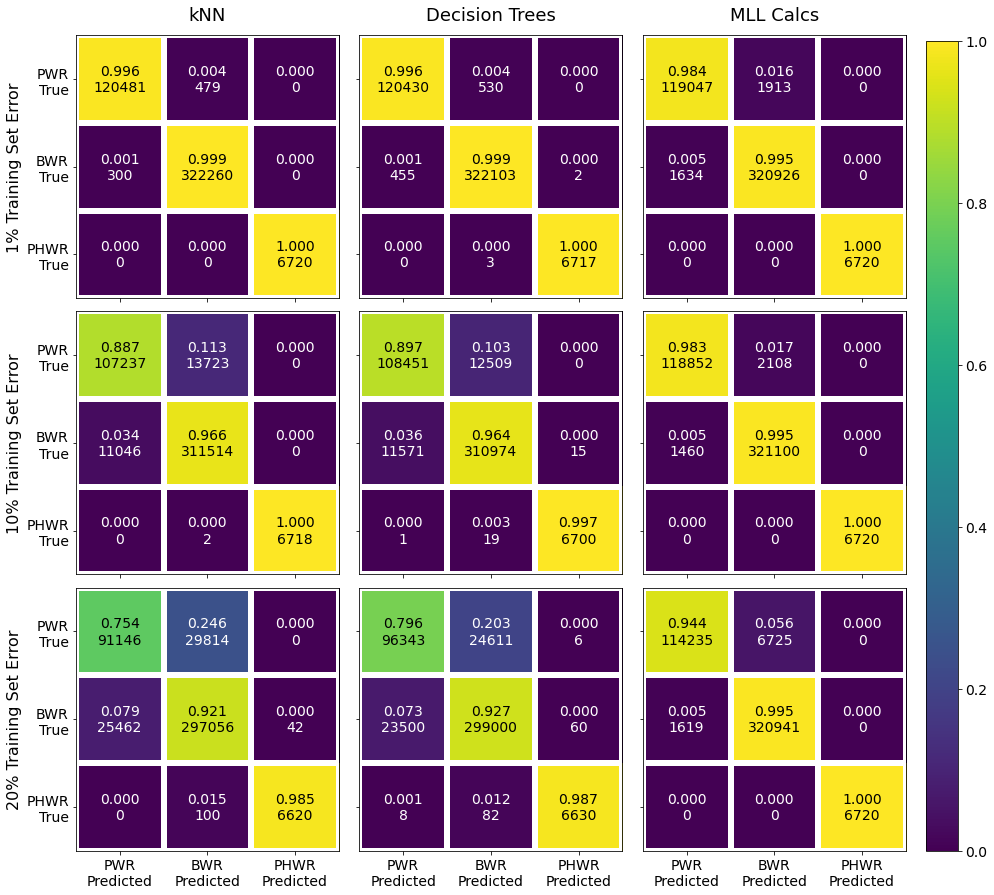
\includegraphics[width=\textwidth]{./chapters/exp1/confusion_matrix_nuc29_3errs.png}
  \caption[Confusion matrices of reactor type classification]
          {Confusion matrices of reactor type prediction for each algorithm 
           at three training set error levels: 1\%, 10\%, and 20\%, in the 
           top, middle, and bottom panels, respectively.}
  \label{fig:cm_nuc29}
\end{figure}

Although the balanced accuracy score provides more information about
classification performance for an imbalanced data set (the training set is
26.8\% \gls{PWR}, 71.6\% \gls{BWR}, and 1.5\% \gls{PHWR}), it still does not
provide much detail about what is being misclassified. To probe this further,
Figure \ref{fig:cm_nuc29} shows three sets of confusion matrices, originally
introduced in Section \ref{sec:testerr}.  The off-diagonal squares are the
fraction of false positives for each reactor type, where the predicted label
(\textit{x}-axis) is something other than the true label (\textit{y}-axis).
The false positive fractions are normalized to the number of true labels.
Below the fractions inside the pixels are the raw numbers of false positives.
The diagonal squares have three numbers in them. The top numbers are the
fraction of true positives for each reactor type (normalized to true labels),
where the predicted label (\textit{x}-axis) is equal to the true label
(\textit{y}-axis).  The middle number in parentheses is the true positive
fraction subtracted by one: $\text{TP} - 1$.  Again, the bottom number is the
raw number of true positives.  

It is ideal to have the diagonal be as close to 1 as possible and the
off-diagonal pixels be as close to 0 as possible.  To allow the fractions to be
rapidly perceived, a colorbar provides perceptually uniform shading for these
true positive and false positive fractions.  The $TP - 1$ along the diagonal is
done so that deviation from perfect classification performance of 1.0 is shaded
a different color (brown) than the off-diagonal pixels that deviate from
perfect classification performance of 0.0 (teal). Perfect performance in both
cases is the middle of the colorbar, white.  

In the top panel of Figure \ref{fig:cm_nuc29}, the three algorithms are
presented for the 1\% random error case. In Figure \ref{fig:randrxtr}, one can
see these three data points on the plot clustered near the top showing
almost-perfect performance.  (A reminder that the true positive fractions in
the confusion matrices do not map directly to the balanced accuracy score,
which puts more weight on the underrepresented classes.) The confusion matrices
give more dimension to this near-perfect reactor type classification
performance. The majority of the misclassification is in \gls{PWR}s being
classified as \gls{BWR}s: 0.4\% for \textit{k}-nearest neighbors and decision
trees, and 1.6\% for \gls{MLL} calculations. Although, there are also some
\gls{BWR}s that are misclassified as \gls{PWR}s: 0.1\% for \textit{k}-nearest
neighbors and decision trees, and 0.5\% for \gls{MLL} calculations.  There are
zero misclassified \gls{PHWR} cases and zero \gls{LWR} cases misclassified as
\gls{PHWR}; the value of 0.000 to three decimals fraction here represents a
real zero-count, but this is not necessarily the case for the other sets of
confusion matrices.  The \gls{PWR}/\gls{BWR} distinction is known to be a
difficult problem, so the correct \gls{PHWR} classifications are not
particularly notable for this discussion. 

The middle panel of Figure \ref{fig:cm_nuc29} shows confusion matrices for the
three algorithms for the 10\% random error case. In Figure \ref{fig:randrxtr},
one can see these three data points on the plot, where the \gls{MLL} point is
near a balanced accuracy score of 1, and the scikit-learn algorithms both have
score of around 0.93. As with the 1\% error case, the majority of the
misclassification is in \gls{PWR}s being classified as \gls{BWR}s: 11.3\% for
\textit{k}-nearest neighbors, 10.3\% for decision trees, and 1.7\% for
\gls{MLL} calculations.  The \gls{BWR}s are being misclassified as \gls{PWR}s
at the following percentages: 3.4\% for \textit{k}-nearest neighbors, 3.6\% for
decision trees, and 0.5\% for \gls{MLL} calculations. Note how the performance
of the \gls{MLL} calculations are nearly the same for both error levels, which
is shown by the \gls{MLL} line in Figure \ref{fig:randrxtr}. Because of the
normalization, the \gls{LWR}s that are misclassified as \gls{PHWR}s appear to
be zero. However, this does happen, just rarely: 15 \gls{BWR}s are classified
as \gls{PHWR} using decision trees. Also, \textit{k}-nearest neighbors and
decision trees misclassified \gls{PHWR} as an \gls{LWR} 2 times using the
former and 20 times using the latter (no \gls{PHWR} misclassifications happened
using \gls{MLL}).

The bottom panel of Figure \ref{fig:cm_nuc29} shows confusion matrices for the
three algorithms for the 20\% random error case. In Figure \ref{fig:randrxtr},
one can see these three data points on the plot, where the \gls{MLL} point is
near a balanced accuracy score of 0.97, \textit{k}-nearest neighbors is around
0.83, and decision trees is around 0.86. As with the previous two error cases,
the majority of the misclassification is in \gls{PWR}s being classified as
\gls{BWR}s: 24.6\% for \textit{k}-nearest neighbors, 20.3\% for decision trees,
and 5.6\% for \gls{MLL} calculations.  The \gls{BWR}s are being misclassified
as \gls{PWR}s at the following percentages: 7.9\% for \textit{k}-nearest
neighbors, 7.3\% for decision trees, and 0.5\% for \gls{MLL} calculations.
\Gls{PHWR}s are misclassified as an \gls{LWR} 100 times for \textit{k}-nearest
neighbors, 82 times for decision trees, and 0 times for \gls{MLL} calculations.
\Gls{LWR}s were misclassified as \gls{PHWR} 42 times for \textit{k}-nearest
neighbors, 66 times for decision trees, and 0 times for \gls{MLL} calculations.

\subsubsection{Regression Results}
\label{sec:randerrB}

Each set of plots for a given prediction parameter in this section shows both
the relative error (\gls{MAPE}) and the absolute error (\gls{MAE}). In addition
to the \gls{MAE} on the second plot for each regression case, the \gls{MedAE}
is represented as a triangle on the plot as well. These three errors taken
together provide more detailed information about the performance of each
algorithm when faced with training set noise.  As previously mentioned, the
\textit{x}-axis has negative errors, so that higher is always better.  

\begin{figure}[!htb]
  \centering
  \begin{subfigure}[b]{0.48\textwidth}
    \centering
    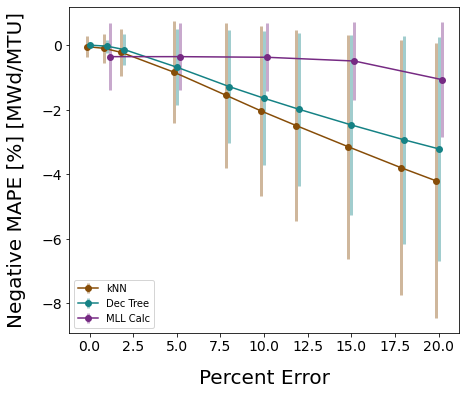
\includegraphics[width=\textwidth]{./chapters/exp1/randerr_compare_nuc29_MAPE_burn.png}
    \caption{Negative \gls{MAPE} of burnup regression with respect to 
             random error.}
    \label{fig:burnmape}
  \end{subfigure}
  \hfill
  \begin{subfigure}[b]{0.5\textwidth}
    \centering
    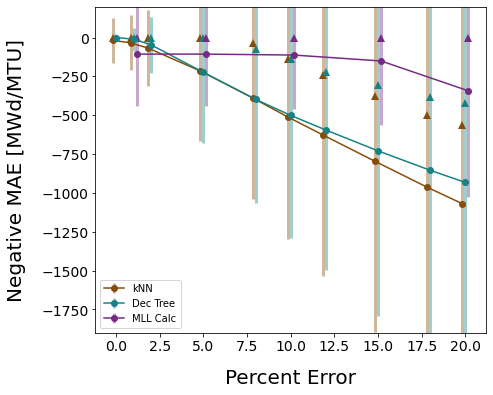
\includegraphics[width=\textwidth]{./chapters/exp1/randerr_compare_nuc29_MAE_burn.png}
    \caption{Negative \gls{MAE} of burnup regression with respect to 
             random error.}
    \label{fig:burnmae}
  \end{subfigure}
  \caption[Prediction performance of burnup regression with increasing training 
           set error]
          {Prediction performance of burnup as measured by relative and 
           absolute errors with respect to uniform/random error applied to the 
           nuclide mass measurements in the training set.}
  \label{fig:randburn}
\end{figure}

Figure \ref{fig:randburn} demonstrates the burnup prediction performance, with
the \gls{MAPE} in Figure \ref{fig:burnmape} and the \gls{MAE} and \gls{MedAE}
in Figure \ref{fig:burnmae}. In these figures, the error bars reflect one
standard deviation of the percentage errors or the absolute errors,
respectively.  As with the reactor type prediction in Figure
\ref{fig:randrxtr}, the \gls{MLL} method is robust to training set error but
performs slightly worse at low error values.  All three methods calculate
burnup with a maximum error of -5\% or $-1000\:MWd/MTU$ at 20\% error in the
training set. The \gls{MedAE}s show a more encouraging picture of the
performance as compared to the \gls{MAE}s. It is interesting that the
scikit-learn algorithms and the \gls{MLL} calculations diverge at 5\% training
set error for \gls{MAPE} and \gls{MAE}, but at 10\% training set error for the
\gls{MedAE}.

\begin{figure}[!htb]
  \centering
  \begin{subfigure}[b]{0.49\textwidth}
    \centering
    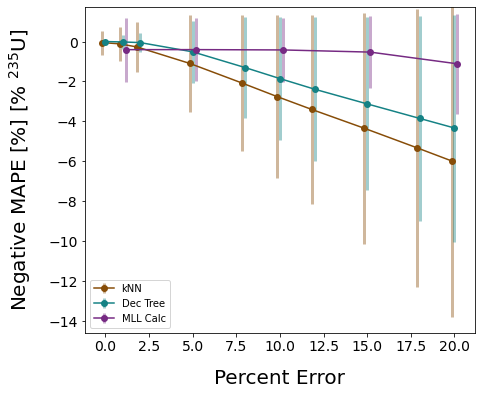
\includegraphics[width=\textwidth]{./chapters/exp1/randerr_compare_nuc29_MAPE_enri.png}
    \caption{Negative \gls{MAPE} of \gls{U235} enrichment regression with 
             respect to random error.}
    \label{fig:enrimape}
  \end{subfigure}
  \hfill
  \begin{subfigure}[b]{0.49\textwidth}
    \centering
    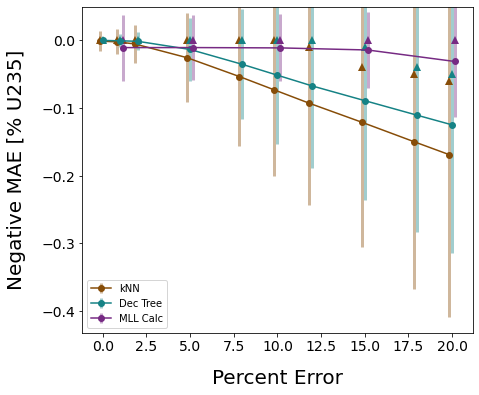
\includegraphics[width=\textwidth]{./chapters/exp1/randerr_compare_nuc29_MAE_enri.png}
    \caption{Negative \gls{MAE} of \gls{U235} enrichment regression with 
             respect to random error.}
    \label{fig:enrimae}
  \end{subfigure}
  \caption[Prediction performance of enrichment regression with increasing 
           training set error]
          {Prediction performance of enrichment as measured by relative and 
           absolute errors with respect to uniform/random error applied to the 
           nuclide mass measurements in the training set.}
  \label{fig:randenri}
\end{figure}  

Figure \ref{fig:randenri} demonstrates the \gls{U235} enrichment prediction
performance, with the \gls{MAPE} in Figure \ref{fig:enrimape} and the \gls{MAE}
and \gls{MedAE} in Figure \ref{fig:enrimae}. In these figures, the error bars
reflect one standard deviation of the percentage errors or the absolute errors,
respectively.  Again, the \gls{MLL} method is robust to training set error but
performs slightly worse at low error values.  All three methods calculate
enrichment with a maximum error of -6\% or $-0.17\:\%U235$ at 20\% error in the
training set. Again, the \gls{MedAE}s show a more encouraging picture of the
performance as compared to the \gls{MAE}s. The scikit-learn algorithms and the
\gls{MLL} calculations diverge at 10\% training set error for \gls{MAPE} and
\gls{MAE}, but at 15\% training set error for the \gls{MedAE}.

\begin{figure}[!htb]
  \centering
  \begin{subfigure}[b]{0.49\textwidth}
    \centering
    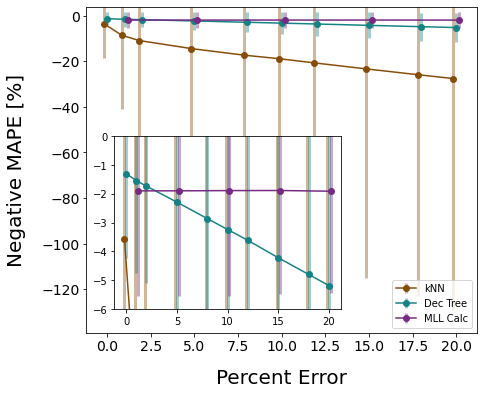
\includegraphics[width=\textwidth]{./chapters/exp1/randerr_compare_nuc29_MAPE_cool.png}
    \caption{Negative \gls{MAPE} of time since irradiation regression with 
             respect to random error.} 
    \label{fig:coolmape}
  \end{subfigure}
  \hfill
  \begin{subfigure}[b]{0.49\textwidth}
    \centering
    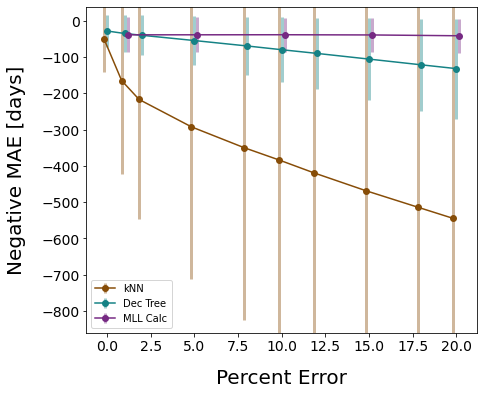
\includegraphics[width=\textwidth]{./chapters/exp1/randerr_compare_nuc29_MAE_cool.png}
    \caption{Negative \gls{MAE} of time since irradiation regression with 
             respect to random error.} 
    \label{fig:coolmae}
  \end{subfigure}
  \caption[Prediction performance of time since irradiation regression with 
           increasing training set error]
          {Prediction performance of time since irradiation as measured by 
           relative and absolute errors with respect to uniform/random error 
           applied to the nuclide mass measurements in the training set.}
  \label{fig:randcool}
\end{figure}

Last, the time since irradiation prediction performance for the three
algorithms with respect to increasing nuclide mass error is pictured in Figure
\ref{fig:randcool}.  The \gls{MAPE} is shown in Figure \ref{fig:enrimape} and
the \gls{MAE} and \gls{MedAE} are shown in Figure \ref{fig:enrimae}.  The error
bars reflect one standard deviation of the percentage errors or the absolute
errors, respectively.  The \gls{MLL} method is most robust to training set
error, but for this prediction parameter, the behavior of \textit{k}-nearest
neighbors is unique here versus the previous two regression categories.  Time
since irradiation is predicted with a maximum error of -30\% or $-550\:days$ at
20\% error in the training set using the \textit{k}-nearest neighbors
algorithm.  In Figure \ref{fig:coolmape}, there is an inset to show more detail
about the behavior of the decision trees and \gls{MLL} calculations curves, so
if one ignores the clearly anomalous \textit{k}-nearest neighbors performance
and focuses instead on decision trees, those values are -6\% and $-120\:days$.
The \gls{MLL} calculations remain nearly horizontal at approximately 2\%
prediction error for all training set error levels.  The \gls{MedAE}, as usual,
shows a more encouraging picture of the performance as compared to the
\gls{MAE}.

Overall, the robustness to training set error that is present in the \gls{MLL}
calculations applies to all of the prediction parameters. The decision trees
performance is second best, and \textit{k}-nearest neighbors performs the
worst.  In the case of time since irradiation, \textit{k}-nearest neighbors
degrades incredibly fast with introduced training set error.  While it is
difficult to draw a baseline for minimum acceptable behavior on these plots,
these performances can serve as a benchmark for the work presented in Chapter
\ref{ch:exp2}. 


\subsubsection{Model Generalization}
\label{sec:randerrC}

Although a key takeaway from Section \ref{sec:randerr} is that the \gls{MLL}
calculations are the most resilient to introduced error in the training set
features for all four prediction categories, there is another aspect of the
algorithm performance not explicitly shown in those plots: generalization.
\Gls{MLL} does not generalize to unseen data; it provides predictions based on
finding the closest training set entry to the test sample.  It (usually)
outperforms the scikit-learn methods in part because the training set is so
large. This is also true for the \textit{k}-nearest neighbor implementations
where $k=1$ (burnup and cooling time, as seen in Table \ref{tbl:exp1hypparam}).

\begin{figure}[!htb]
  \centering
  \begin{subfigure}[b]{0.495\textwidth}
    \centering
    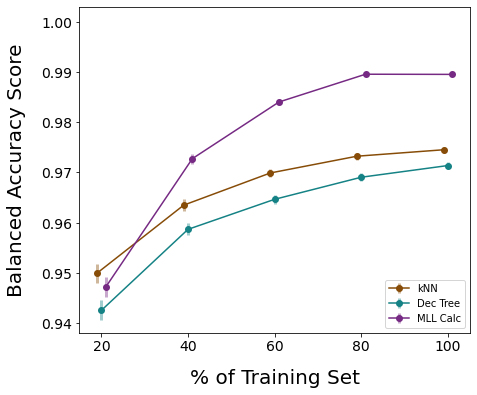
\includegraphics[width=\textwidth]{./chapters/exp1/learncurve_nuc29_err05_BalAcc_rxtr.png}
    \caption{Balanced accuracy of reactor type classification with respect 
             to training set size.}
    \label{fig:learnsA}
  \end{subfigure}
  \hfill
  \begin{subfigure}[b]{0.485\textwidth}
    \centering
    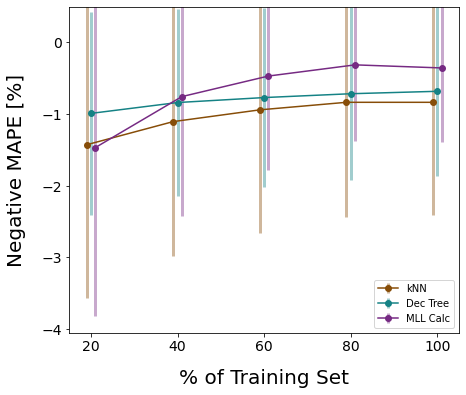
\includegraphics[width=\textwidth]{./chapters/exp1/learncurve_nuc29_err05_MAPE_burn.png}
    \caption{Negative \gls{MAPE} of burnup regression with respect to 
             to training set size.}
    \label{fig:learnsB}
  \end{subfigure}
  \vskip\baselineskip
  \begin{subfigure}[b]{0.48\textwidth}
    \centering
    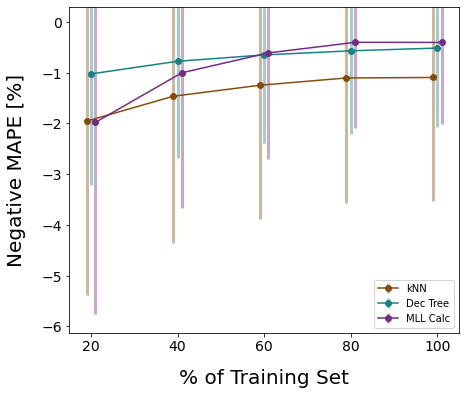
\includegraphics[width=\textwidth]{./chapters/exp1/learncurve_nuc29_err05_MAPE_enri.png}
    \caption{Negative \gls{MAPE} of \gls{U235} enrichment regression with 
             respect to training set size.}
    \label{fig:learnsC}
  \end{subfigure}
  \hfill
  \begin{subfigure}[b]{0.50\textwidth}
    \centering
    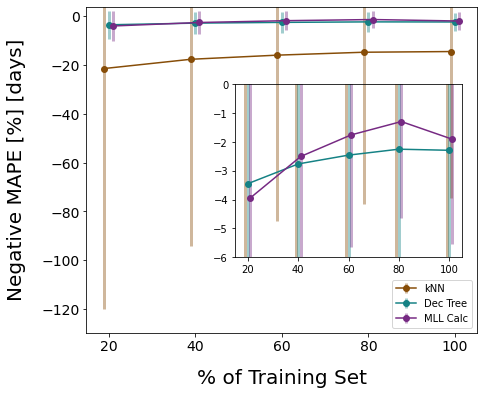
\includegraphics[width=\textwidth]{./chapters/exp1/learncurve_nuc29_err05_MAPE_cool.png}
    \caption{Negative \gls{MAPE} of time since irradiation regression with 
             respect to training set size.}
    \label{fig:learnsD}
  \end{subfigure}
  \caption[Learning curves for all four prediction parameters]
          {Learning curves for reactor type, burnup, enrichment, and time 
           since irradiation with respect to increasing fraction of the 
           training set, for 5\% training set random error.}
  \label{fig:learns}
\end{figure}

One way to show that an algorithm is generalizing well in comparison to others
is to view the shape of its learning curve (introduced in Section
\ref{sec:complexity}): the prediction performance with respect to training set
size.  It is crucial to have the training sets be identical for each algorithm,
so they were created in advance and the learning curves are constructed
manually rather than relying on the scikit-learn method.  Smaller training sets
were created from the original one by taking 80\%, 60\%, 40\%, and 20\% of the
entries. The training sets are all stratified so that the original fractions of
\gls{BWR}, \gls{PWR}, and \gls{PHWR} are retained. They are also built on top
of one another, so the 20\%-size training set is contained within the 40\%-size
set, and so forth.

Learning curves were constructed for all four prediction categories,
demonstrated in Figure \ref{fig:learns}. As in Figures
\ref{fig:randrxtr}--\ref{fig:randcool} , the vertical axis is always oriented
so that lower is poorer performance and higher is better performance; also, the
error bars reflect a 99\% confidence interval for Figure \ref{fig:learnsA}, and
one standard deviation of the average percentage errors for Figures
\ref{fig:learnsB}--\ref{fig:learnsD}.  These learning curves represent the 5\%
random error case in Figures \ref{fig:randrxtr}--\ref{fig:randcool}, so the
scores/errors in these figures are the data points at the 100\% training set
level in Figure \ref{fig:learns}.  Therefore, the leftmost data in Figure
\ref{fig:learns} will show the \gls{MLL} point being slightly above the
scikit-learn points for the reactor type, burnup, and enrichment predictions,
and the \textit{k}-nearest neighbor point is below the \gls{MLL} and decision
trees points for time since irradiation.  

Figure \ref{fig:learnsA} shows that the balanced accuracy score of reactor type
classification for the \gls{MLL} calculations decreases more at lower training
set size than for the scikit-learn algorithms. Here, the curve crosses below
the \textit{k}-nearest neighbors curve at the lowest training set size of 20\%.
For the burnup \gls{MAPE} in Figure \ref{fig:learnsB} and the enrichment
\gls{MAPE} in Figure \ref{fig:learnsC}, the \gls{MLL} curve crosses below both
of the scikit-learn algorithm curves. This happens between 20\% and 40\%
training set size for burnup, and between 40\% and 60\% training set size for
enrichment.  Lastly, Figure \ref{fig:learnsD} shows a different arrangement,
which is to be expected from the results shown in Figure \ref{fig:randcool},
where the \textit{k}-nearest neighbors performance is significantly worse than
the other two algorithms. Because the \textit{k}-nearest neighbors curve and
error bars are so large, there is an inset showing a closeup of the other two
curves above -6\%.  The decision trees and \gls{MLL} calculations curves now
appear to follow the trend in the burnup and enrichment cases, and the
\gls{MLL} curve crosses under the decision trees curve between 20\% and 40\%
training set size.  

There is a dependence on training set size for all three algorithms in Figure
\ref{fig:learns}. For the most part, the \textit{k}-nearest neighbors and
decision trees curves follow an approximately parallel path, whereas the
\gls{MLL} method shows an increased rate of degradation at low training set
sizes. Since this training set is large enough, i.e., the prediction parameters
were included in small enough steps, that \gls{MLL} has consistent performance
at the larger sizes, there is not a concern in this work about its inability to
generalize. It must be noted, however, that the \gls{MLL} approach requires a
fine grid of simulation parameters in a training database to perform better
than the simple scikit-learn algorithms.

\subsubsection{Reactor Type Prior Knowledge}
\label{sec:randerrD}

There is similar work being done to this work that focuses on similar
prediction categories but in a serial manner, i.e., first determining the
reactor type before moving forward with other predictions \cite{serial_ml}.
This work predicts reactor operation parameters while blind to the reactor
type, but it makes sense intuitively that having previous knowledge of the
reactor type would allow more accurate regression of these parameters.
Therefore, the change in regression performance from the reactor type-blind
predictions to having prior knowledge of the reactor type is discussed.

The workflow was repeated for the three regression cases where they were
trained on reactor type-specific training sets. A 5\% random error was applied
to these training sets, and the 5\% random error full training set was used as
comparison. The errors for each algorithm (\textit{k}-nearest neighbors,
decision trees, and \gls{MLL} calculations) were tallied for each regression
category (burnup, enrichment, and time since irradiation) and within that, for
each reactor type (\gls{PWR}, \gls{BWR}, \gls{PHWR}). Two sets of error were
tracked: whether the reactor type was \textit{known} or \textit{unknown} prior
to prediction.

Table \ref{tbl:knownrxtr} shows the \gls{MAPE}s for each regression category
and within that, for each reactor type (\gls{PWR}, \gls{BWR}, \gls{PHWR}).  The
columns are separated first by the algorithms and second by whether the reactor
type was known or unknown prior to prediction, denoted as \textit{K} and
\textit{U}, respectively. Most of these relative errors are quite low, and
around or under 2\%.  So, e.g., despite burnup prediction from \glspl{PHWR}s
improving, it was by 0.61\%, a precision of which may not be of concern. Still,
these performance differences can be looked at in more detail.  

\begin{table}[!htb]
  \centering
  \begin{tabular}{@{}llllllll@{}}
    \toprule
    &  &  \multicolumn{2}{c}{\textit{k}NN} 
    &     \multicolumn{2}{c}{Dec Trees} 
    &     \multicolumn{2}{c}{MLL Calcs} \\ 
    \toprule
    \begin{tabular}[c]{@{}l@{}}Prediction\\ Parameter\end{tabular} &
    \begin{tabular}[c]{@{}l@{}}Reactor \\ Type\end{tabular} &
    K & U &  K & U & K & U \\ \midrule
    \multirow{3}{*}{\begin{tabular}[c]{@{}l@{}}Burnup \\ \% {$[MWd/MTU]$} \end{tabular}}
     & PWR  & 0.60  & 0.66  & 0.54 & 0.75 & 0.24 & 0.25 \\
     & BWR  & 0.88  & 0.90  & 0.60 & 0.66 & 0.40 & 0.40 \\
     & PHWR & 0.66  & 1.27  & 0.14 & 0.54 & 0.28 & 0.28 \\ \hline
    \multirow{3}{*}{\begin{tabular}[c]{@{}l@{}}Enrichment \\ \% {$[\%\:{}^{235}\text{U}]$} \end{tabular}}
     & PWR  & 0.85  & 0.99  & 0.36 & 0.48 & 0.26 & 0.29 \\
     & BWR  & 1.14  & 1.16  & 0.51 & 0.54 & 0.45 & 0.46 \\
     & PHWR & 0.00  & 0.00  & 0.00 & 0.02 & 0.00 & 0.00 \\ \hline
    \multirow{3}{*}{\begin{tabular}[c]{@{}l@{}}Time Since \\ Irradiation \\ \% {$[days]$} \end{tabular}}
     & PWR  & 11.44 & 10.48 & 2.35 & 2.19 & 1.55 & 1.46 \\
     & BWR  & 15.39 & 15.48 & 2.27 & 2.28 & 2.06 & 2.05 \\
     & PHWR & 19.32 & 34.41 & 4.96 & 4.52 & 2.30 & 2.30 \\ \bottomrule
  \end{tabular}
  \caption[\acrshort{MAPE}s for three regression cases comparing known versus 
           unknown reactor type prior knowledge]
          {\acrshort{MAPE}s for the three prediction cases for each algorithm 
           at 5\% training set error. \textit{K} refers to \textit{known} 
           reactor type and \textit{U} refers to \textit{unknown} reactor type 
           prior to regression.}
  \label{tbl:knownrxtr}
\end{table}

To better see these performance differences, the percent change in prediction
\gls{MAE} for each algorithm and reactor type between the reactor type being
known versus unknown prior to prediction was calculated as: $100 \cdot
\frac{MAE_{unknown} - MAE_{known}}{MAE_{unknown}}$.  This was chosen to be
relative to the unknown error since that is the benchmark in this case.  Figure
\ref{fig:knownrxtr} is three heatmaps that show this percent change for each
prediction category, algorithm, and reactor type.  This value is reflected by a
diverging color bar as well as a positive or negative percentage in each
square.  The positive percentages indicate the error decreased/improved from
the unknown reactor type case to the known reactor type case.  The negative
percentages indicate the error increased/worsened from the unknown to the known
case. 

\begin{figure}[!htb]
  \centering
  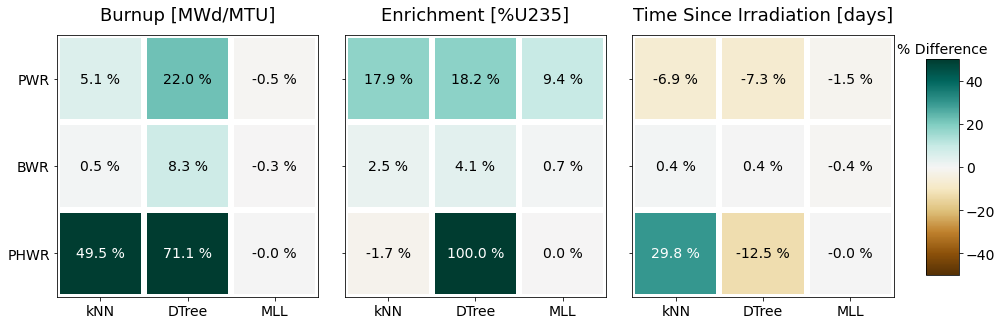
\includegraphics[width=\textwidth]{./chapters/exp1/rxtr-type_known-unknown_diff_err05.png}
  \caption[Heatmaps for three regression cases comparing known versus 
           unknown reactor type prior knowledge]
          {Heatmaps for the three regression cases showing the percent 
           difference in prediction error between a known reactor type 
           and unknown reactor type using a 5\% training set error.}
  \todo[inline]{would this be better shown with a plot that has little arrows? or leave like this?}
  \label{fig:knownrxtr}
\end{figure}

For burnup prediction, most differences are within $\pm10\%$ except for three
scenarios.  The decision tree algorithm has improved burnup prediction for
\glspl{PWR}s by 22.0\% and for \glspl{PHWR}s by 71.1\% given a known reactor
type.  The \textit{k}-nearest neighbors algorithm has 49.5\% improved burnup
prediction for the \gls{PHWR}. For \gls{U235} enrichment, the \gls{PWR}
predictions improve by approximately 18\% for the scikit-learn algorithms.
Even though the value is within $\pm10\%$, this is the only scenario where
there is an appreciable difference in \gls{MLL} performance. The decision tree
enrichment prediction of \glspl{PHWR}s also has a sizeable improvement of
100.0\%.  The time since irradiation predictions for the most part do not show
improvement outside of $\pm10\%$. Of note is some volatile behavior for the
\gls{PHWR} case with the scikit-learn algorithms.  While \textit{k}-nearest
neighbors improves by 29.8\%, the decision tree predictions were worse by
12.5\%.  Since the main concern here is showing how prediction performance
improves with prior reactor type knowledge, this reduction in performance is
odd but not worthy of further investigation.

The improvements in the \gls{PHWR} predictions are not surprising since the
generalization of the scikit-learn algorithms could lead to the unique
\gls{PHWR} cases being ignored, since they are after all only 1.5\% of the
training set.  Another interesting result is that the \gls{BWR} predictions
experience no large changes, which makes sense given that they comprise 72\% of
the training set. Also, the \gls{MLL} predictions are approximately the same,
which is expected because this algorithm does not generalize, and the
prediction comes as a set of labels and is therefore already linked to the
reactor type. Overall, it is important to be aware that the regression labels
coming from a \gls{PHWR} will be unlikely to be optimal results (except for
those from \gls{MLL} calculations).

%\begin{table}[!htb]
%  \centering
%  \begin{tabular}{@{}llllllll@{}}
%    \toprule
%    &  &  \multicolumn{2}{c}{\textit{k}NN} 
%    &     \multicolumn{2}{c}{Dec Trees} 
%    &     \multicolumn{2}{c}{MLL Calcs} \\ 
%    \toprule
%    \begin{tabular}[c]{@{}l@{}}Prediction\\ Parameter\end{tabular} &
%    \begin{tabular}[c]{@{}l@{}}Reactor \\ Type\end{tabular} &
%    K & U &  K & U & K & U \\ \midrule
%    \multirow{3}{*}{\begin{tabular}[c]{@{}l@{}}Burnup \\ \% {$[MWd/MTU]$} \end{tabular}}
%     & PWR  & 0.08  & 0.08  & 0.03 & 0.04 & 0.24 & 0.25 \\ 
%     & BWR  & 0.11  & 0.10  & 0.03 & 0.03 & 0.40 & 0.40 \\ 
%     & PHWR & 0.13  & 0.19  & 0.01 & 0.03 & 0.29 & 0.29 \\ \hline
%    \multirow{3}{*}{\begin{tabular}[c]{@{}l@{}}Enrichment \\ \% {$[\%\:{}^{235}\text{U}]$} \end{tabular}}
%     & PWR  & 0.10  & 0.11  & 0.02 & 0.02 & 0.26 & 0.29 \\ 
%     & BWR  & 0.12  & 0.12  & 0.02 & 0.02 & 0.46 & 0.46 \\ 
%     & PHWR & 0.00  & 0.00  & 0.00 & 0.00 & 0.00 & 0.00 \\ \hline
%    \multirow{3}{*}{\begin{tabular}[c]{@{}l@{}}Time Since \\ Irradiation \\ \% {$[days]$} \end{tabular}}
%     & PWR  & 6.47  & 6.13  & 1.50 & 1.43 & 1.55 & 1.46 \\ 
%     & BWR  & 9.18  & 9.15  & 1.56 & 1.53 & 2.07 & 2.05 \\ 
%     & PHWR & 13.78 & 18.62 & 4.51 & 3.71 & 2.30 & 2.30 \\ \bottomrule
%  \end{tabular}
%  \caption{\gls{MAPE}s for the three prediction cases for each algorithm at 1\% 
%           training set error. \textit{K} refers to \textit{known} reactor 
%           type and \textit{U} refers to \textit{unknown} reactor type prior 
%           to regression.}
%  \label{tbl:knownrxtr}
%\end{table}

%\begin{figure}[!htb]
%  \centering
%  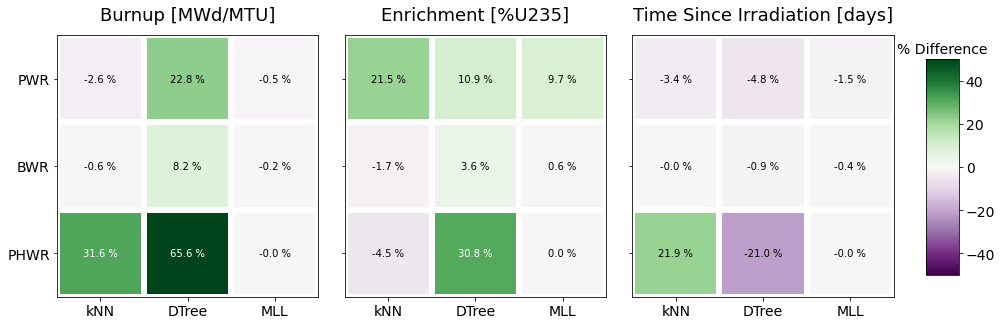
\includegraphics[width=\textwidth]{./chapters/exp1/rxtr-type_known-unknown_diff_err01.png}
%  \caption{Heatmaps for the three regression cases showing the percent 
%           difference in prediction error between a known reactor type 
%           and unknown reactor type.}
%  \label{fig:knownrxtr}
%\end{figure}



\subsection{SFCOMPO Test Set}
\label{sec:sfcompo}

\todo[inline]{1. all of my commentary on performance improvement for the
sfcompo test set is outlined to go into the future work section. or should it
go here?  2. also, there may be some useful information from the model
generalization or rxtr type prior knowledge sections that could be useful here
for more in depth discussion. 3. this ended up really motivating the use of
relative error versus absolute (really, both) so it could maybe go first, then
the random error results section could go second using the relative error
plots?}

The testing described in Section \ref{sec:randerr} describes the process of
evaluating the methodology with test cases drawn from the training database.
It is also helpful to test the methodology against real assays of \gls{SNF}.
The \gls{SFCOMPO} database was created to allow access to these sorts of
measurements linked to the reactor operation parameters being predicted in this
work. \cite{sfcompo}. The only parameter not part of the \gls{SFCOMPO} database
is the time since irradiation, so that is not predicted here. 

\begin{figure}[!htb]
  \centering
  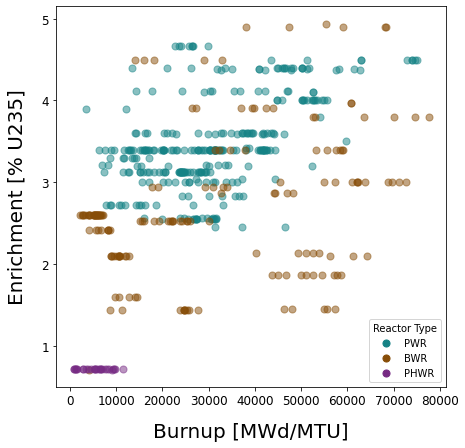
\includegraphics[width=0.7\textwidth]{./chapters/exp1/sfcompo_scatter_viz.png}
  \caption{Scatter plot showing the range of reactor operation parameters in 
           the \gls{SFCOMPO} testing set that are being predicted.}
  \label{fig:sfcoscatter}
  \todo[inline]{maybe show comparison against training E v B scatter plot}
\end{figure}

There are 505 test cases that are able to be compared against the training
database.  The number of each reactor type is as follows: 312 \gls{PWR}s, 165
\gls{BWR}s, and 28 \gls{PHWR}s. The space of enrichment and burnup values is
visualized in Figure \ref{fig:sfcoscatter}. These are sufficiently represented
in the training set design, as pictured in Figure \ref{fig:trainhist}, although
the proportions of \gls{PWR} and \gls{BWR} are approximately opposite to the
training set. The assays in \gls{SFCOMPO} are presented as nuclide
concentrations with the units \textit{milligrams per grams of initial uranium},
or $mg/gU_i$. The training set of nuclide measurements in \textit{grams} is
converted to these concentration units prior to prediction is converted to
these concentration units prior to prediction. 

There is one main issue with using \gls{SFCOMPO} as a testing set: missing
nuclide measurements.  The feature set of 29 nuclides in Table
\ref{tbl:nucmass} was chosen based on the frequency of these measurements being
present in the database at an arbitrary level of 100 measurements. This
happened before filtering, so there are some nuclide measurements present at
under 100 counts.  Each nuclide's frequency in \gls{SFCOMPO} is listed in Table
\ref{tbl:missing}.  While every assay contains several plutonium measurements
and most contain uranium measurements as well, the remaining nuclides are
present at a much lower rate. 

\begin{table}[!htb]
  \centering
  \begin{tabular}{>{\raggedleft}m{0.6in}
                                m{0.4in}
                  >{\raggedleft}m{0.6in}
                                m{0.4in}
                  >{\raggedleft}m{0.6in}
                                m{0.4in}}
    \toprule
    \rowcolor[gray]{0.88} am241  & 237 & nd145 & 162 & sm147 & 97  \\  
    \rowcolor[gray]{0.95} am242m & 110 & nd146 & 139 & sm149 & 97  \\ 
    \rowcolor[gray]{0.88} am243  & 203 & nd148 & 275 & sm150 & 97  \\ 
    \rowcolor[gray]{0.95} cm242  & 214 & nd150 & 121 & sm151 & 97  \\ 
    \rowcolor[gray]{0.88} cm244  & 269 & np237 & 155 & sm152 & 97  \\ 
    \rowcolor[gray]{0.95} cs134  & 113 & pu238 & 369 & u234  & 355 \\ 
    \rowcolor[gray]{0.88} cs137  & 185 & pu239 & 505 & u235  & 479 \\ 
    \rowcolor[gray]{0.95} eu154  & 100 & pu240 & 505 & u236  & 462 \\ 
    \rowcolor[gray]{0.88} nd143  & 162 & pu241 & 504 & u238  & 433 \\ 
    \rowcolor[gray]{0.95} nd144  & 113 & pu242 & 505 &       &     \\ \bottomrule
  \end{tabular}
  \caption{Number of assays each nuclide is measured for in the \gls{SFCOMPO}
           database.}
  \label{tbl:missing}
\end{table}

Although some algorithms in theory can handle null values in the training
stage, scikit-learn does not currently include this capability. The \gls{MLL}
method is designed to handle null values, however. This is done by converting
them to zero and filtering out all zero-valued nuclides during the likelihood
calculations. But there is a technique more commonly applied than converting
missing values to zero: imputation. This involves taking the mean or median of
the existing features and applying that value to the assays in which it is
missing.  The remainder of this section dicusses using the three algorithms to
predict the \gls{SFCOMPO} test cases where the nulls are both converted to zero
and imputed using the mean.  \todo[inline]{is converting to zero technically
imputation as well?}

\subsubsection{Reactor Type Classification}

Table \ref{tbl:sfcorxtr} presents two metrics for the two missing value
techniques: the accuracy and balanced accuracy scores. The accuracy scores for
both the imputed nulls and zero-nulls test sets are mostly under 0.62, which is
the fraction of \gls{PWR} entries.  Therefore, a classifier could predict
\gls{PWR} every time and do better than these accuracy scores.  For the
zero-nulls test set predictions using \gls{MLL}, however, the accuracy of 0.72
does exceed the "majority guess" accuracy of 0.62.  Since \gls{MLL}
calculations filter out null values, it is expected that the scores will be
higher for all prediction categories where \gls{MLL} is being used with the
zero-nulls test set. This expected \gls{MLL} performance also holds true when
looking at the balanced accuracy score.  A balanced accuracy score of 0 denotes
random guessing, but it can also be negative if the classifications are worse
than random guessing. The balanced accuracy of 0.63 for the zero-nulls case is
a promising result. The balanced accuracies of \textit{k}-nearest neighbors and
decision trees are all quite low. Also, the higher accuracies correspond to lower
balanced accuracies, and vice versa. Therefore, further investigation is
necessary.

\begin{table}[!htb]
  \centering
  \begin{tabular}{@{}m{1.5in}llllll@{}}
    \toprule
    & \multicolumn{3}{m{2in}}{Accuracy Scores} 
    & \multicolumn{3}{l}{Balanced Accuracy Scores} \\ 
    \toprule
    Null Handling    & kNN   & DTree  & MLL   & kNN   & DTree  & MLL    \\ \midrule
    Imputed Nulls    & 0.52  & 0.60   & 0.39  & 0.09  & 0.12   & -0.01  \\
    Zero-value Nulls & 0.45  & 0.42   & 0.72  & 0.21  & 0.30   & 0.63   \\ \bottomrule
    \end{tabular}
  \caption{Accuracy and balanced accuracy scores for reactor type prediction 
           of the \gls{SFCOMPO} test cases.}
  \label{tbl:sfcorxtr}
\end{table}

\begin{figure}[!htb]
  \centering
  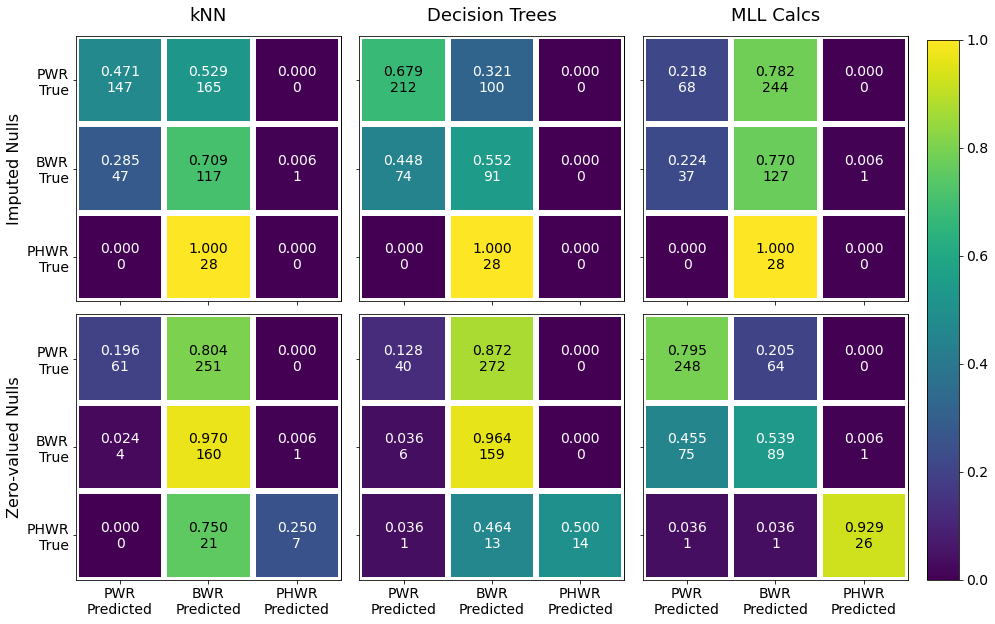
\includegraphics[width=\textwidth]{./chapters/exp1/confusion_matrix_sfco.png}
  \caption{Confusion matrices of reactor type prediction for each algorithm 
           using two missing entry techniques: imputation with mean values (top 
           panel) and replacement with zero (bottom panel).}
  \label{fig:cm}
\end{figure}

Figure \ref{fig:cm} allows for a deeper look into what is happening with the
reactor type predictions for both of the \gls{SFCOMPO} test sets.  The matrices
from using mean-imputed null values are in the top panel and the matrices from
using zero-filled null values are in the bottom panel.  The scikit-learn
algorithms have a higher accuracy for the imputed null values test set than
their zero-null values counterparts, but the balanced accuracies follow the
opposite direction. For \textit{k}-nearest neighbors, imputed nulls cause more
than half of the \gls{PWR}s and all of the \gls{PHWR}s to be misclassified as
\gls{BWR}s. Additionally, 28.5\% \gls{BWR}s are misclassified as \gls{PWR}s.
For the zero-nulls test set, there is a much larger correct \gls{BWR}
classification percentage, but also a much larger \gls{PWR} misclassification
percentage. The \gls{PHWR} true positive percentage increases from 0 to 25\%.
\Gls{BWR} (32\% of test cases) and \gls{PHWR} (5.5\% of test cases) are the two
minority classes in the database.  Because they both have higher true positive
fractions but there were overall fewer correct predictions (from a much higher
\gls{PWR} misclassification) from the imputed nulls to the zero-nulls, the
accuracy went down but the balanced accuracy went up.

Decision trees follows a similar pattern the the \textit{k}-nearest neighbors
example.  The \gls{PWR} misclassification increases from the imputed nulls to
the zero-nulls test set in a similar manner, although the original \gls{PWR}
true positive fraction is higher (leading to a higher accuracy for the imputed
nulls case).  As before, the \gls{BWR} correct classification increases
drastically from the imputed nulls to zero-nulls case.  Additionally, the
\gls{PHWR} classifiction improvement from imputed nulls to zero-nulls is better
for decision trees than for \textit{k}-nearest neighbors.  Therefore, again,
the accuracy decreased and the balanced accuracy increased. The larger
improvement for the minority classes has led to the larger balanced accuracy
improvement for decision trees.

In Figure \ref{fig:cm}, the confusion matrices for the \gls{MLL} calculations
tell a very different story than those for the scikit-learn algorithms.  The
only similarity is that using imputed nulls causes all \gls{PHWR}s to be
classified as \gls{BWR}s. \gls{PWR}s are misclassified as \gls{BWR}s at 78.2\%,
and \gls{BWR}s are misclassified as \gls{PWR}s at 22.4\%. For the zero-nulls
test set, \gls{PHWR}s and \gls{PWR}s true positive percentages sharply improve
to 92.9\% and 79.5\%, respectively.  The true positive rate for \gls{BWR}s,
however, decreases from 77.0\% to 53.9\%. This is the opposite trend from both
of the scikit-learn algorithms.  Despite the misclassification increase for
\gls{BWR}s, both the accuracy score and balanced accuracy score increase for
\gls{MLL} calculations when moving from using imputed null values to zero-null
values in the test set. The improvement in \gls{MLL} classification is likely
because the imputed nulls test set hides information rather than removing it
from consideration, which is what the zero-nulls test set does. 

All three algorithms using both test sets tend towards misclassifying
\gls{PHWR}s as \gls{BWR}s (except for \gls{MLL} calculations using zero-null
missing values).  This is likely because \gls{BWR}s comprise the majority of
the training set (72\%), and no matter how the missing measurements are handled
there may be too little information to predict these well with most algorithms.
For the two scikit-learn algorithms, the zero-nulls test set predicts
\gls{BWR}s the majority of the time (despite there being 50\% correct
\gls{PHWR} prediction for decision trees). This also is likely from \gls{BWR}
being the training set majority class, so with many nuclides measuring at zero,
there are likely to be few good matches, and the majority class becomes the
most likely prediction. This explanation is possibly applicable to the imputed
nulls test set as well, but the behavior pattern is less clear because the
imputed nulls give more information for these algorithms than zero-value nulls
(since the zero-values cannot be removed from consideration), so a larger
proportion of \gls{PWR}s are being predicted properly.  \todo[inline]{look up
paper that uses only U/Pu to predict, because that would be the only way these
505 cases would be able to be predicted without having so much missing
information. MLL essentially does this for 0 null case which is why it does
better than the rest}

\subsubsection{Regression Cases}

Next, the prediction of \gls{SFCOMPO} test samples for the regression cases
will be discussed. There is no time since irradiation value in the database, so
only burnup and \gls{U235} enrichment are discussed here.  While the mean and
median errors for burnup and enrichment prediction are listed in Tables
\ref{tbl:sfcoburn} and \ref{tbl:sfcoenri}, respectively, there are also box
plots inlcuded for both absolute and relative errors in Figures
\ref{fig:sfcoburn} and \ref{fig:sfcoenri}, respectively.  Box plots were chosen
since they can provide a larger amount of information than just a mean or
median value.  The white triangles represent the mean error, and the white line
in notched box is the median error. The box itself is the 25\% (Q1) and 75\%
(Q3) quartiles at the bottom and top, respectively. The error bars or whiskers
are meant to represent the spread of all errors minus the outliers.  The bottom
whisker reaches to $Q1 - 1.5*(Q3-Q1)$ and the top whisker reaches to $Q3 +
1.5*(Q3-Q1)$. Any values outside of this range are considered outliers.
\cite{matplotlib}

\noindent \textbf{Burnup}

The expected results that \gls{MLL} will perform better with the zero-nulls
test set also holds true for the regression cases, as shown in Table
\ref{tbl:sfcoburn}.  While the scikit-learn algorithms have a moderate increase
in both the mean and median burnup errors from the imputed nulls to the
zero-nulls, the \gls{MLL} calculations have an order of magnitude decrease in
error when moving in that same direction.  Seeing this trend between Figures
\ref{fig:burnimp} and \ref{fig:burn0} is a little difficult due to the
different ranges on the \textit{y}-axes, but the drastic improvement in
\gls{MLL} burnup error from the imputed nulls in Figure \ref{fig:burnimp} to
the zero-nulls in Figure \ref{fig:burn0} is still visually clear. In the latter
figure, there is one outlier for \textit{k}-nearest neighbors and 39 for
\gls{MLL} calculations.

\begin{table}[!htb]
  \centering
  \begin{tabular}{@{}m{1.5in}llllll@{}}
    \toprule
                     & \multicolumn{3}{m{2in}}{Mean Errors [GWd/MTU]} & \multicolumn{3}{c}{Median Errors [GWd/MTU]} \\ \toprule
    Null Handling    & kNN           & DTree         & MLL           & kNN            & DTree          & MLL    \\ \midrule
    Imputed Nulls    & 9.43          & 10.89         & 13.17         & 7.26           & 8.28           & 10.84  \\
    Zero-value Nulls & 14.88         & 15.18         & 3.53          & 11.47          & 8.79           & 1.70   \\ \bottomrule
  \end{tabular}
  \caption{Mean and median errors for burnup prediction of the \gls{SFCOMPO} 
           test cases.}
  \label{tbl:sfcoburn}
\end{table}

Although the mean and median errors are contained in the range of $1-15
GWd/MTU$, the large spread in burnup errors in Figures \ref{fig:burnimp} and
\ref{fig:burn0} for all three algorithms was broad enough to warrant an
investigation into the range of relative errors, expressed as percent errors in
Figures \ref{fig:burnimppct} and \ref{fig:burn0pct}.  In Figure
\ref{fig:burnimppct} there are 75, 72, and 73 outliers (all around 15\% of the
test database) for the \textit{k}-nearest neighbors, decision trees, and
\gls{MLL} calculations, respectively.  In Figure \ref{fig:burn0pct} there are
45 outliers for the \gls{MLL} calculations.

\begin{figure}[!htb]
  \centering
  \begin{subfigure}[b]{0.49\textwidth}
    \centering
    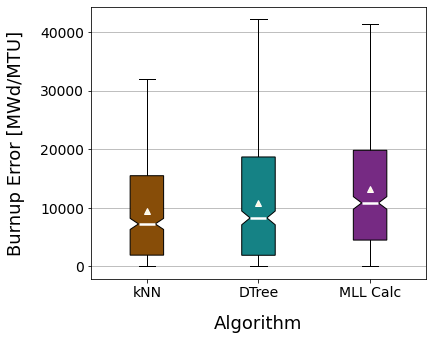
\includegraphics[width=\textwidth]{./chapters/exp1/sfcompo_boxplots_impnull_burn.png}
    \caption{Box plots of burnup errors using mean-imputed null values.}
    \label{fig:burnimp}
  \end{subfigure}
  \hfill
  \begin{subfigure}[b]{0.49\textwidth}
    \centering
    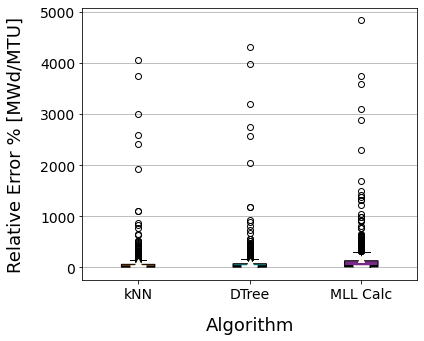
\includegraphics[width=\textwidth]{./chapters/exp1/sfcompo_boxplots_impnull_pcterr_burn.png}
    \caption{Box plots of burnup percentage errors using mean-imputed null values.}
    \label{fig:burnimppct}
  \end{subfigure}
  \vskip\baselineskip
  \begin{subfigure}[b]{0.49\textwidth}
    \centering
    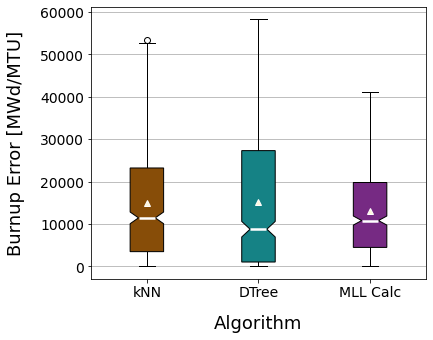
\includegraphics[width=\textwidth]{./chapters/exp1/sfcompo_boxplots_0null_burn.png}
    \caption{Box plots of burnup errors using zero-replaced null values.}
    \label{fig:burn0}
  \end{subfigure}
  \hfill
  \begin{subfigure}[b]{0.49\textwidth}
    \centering
    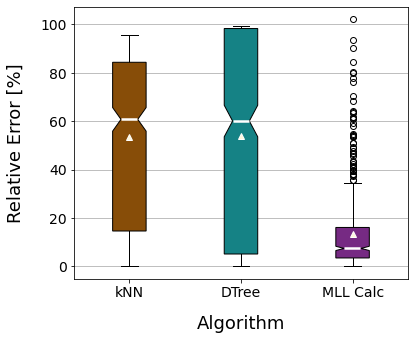
\includegraphics[width=\textwidth]{./chapters/exp1/sfcompo_boxplots_0null_pcterr_burn.png}
    \caption{Box plots of burnup percentage errors using zero-replaced null values.}
    \label{fig:burn0pct}
  \end{subfigure}
  \caption{Box plots of burnup prediction errors and percentage errors for each 
           algorithm using two missing entry techniques: imputation with mean 
           values and replacement with zero.}
  \label{fig:sfcoburn}
\end{figure}

The ranges seen for the imputed nulls test set in Figure \ref{fig:burnimppct}
are as large as they are from low burnups ($< 10 GWd/MTU$) being far
overpredicted, since a small number in the denominator will yield a high
percentage error. A large subset of the low burnup cases are \gls{PHWR}s.
Their burnups are also unlikely to be predicted well because of the inability
of \gls{PHWR} reactors to be represented accurately with this methodology.
Removing the \gls{PHWR} reactors from the results removes all outliers with
percentage errors larger than 1750\%. That is still a very high relative error,
but there are other low burnup cases in the database.  Removing \gls{PHWR}s
does not significantly alter the zero-nulls results in Figure
\ref{fig:burn0pct}.

The range of percentage errors for the zero-nulls test set in Figure
\ref{fig:burn0pct} tells a different story. There is only one case (an
\gls{MLL} outlier) that is above 100\% error.  While the absolute errors for
the scikit-learn algorithms in Figure \ref{fig:burn0} span a larger range than
their counterparts in Figure \ref{fig:burnimp}, their relative errors remain
within $0-100\%$. The only case that predicts the burnup well is the \gls{MLL}
method with the zero-null missing values treatment of the \gls{SFCOMPO} test
set, but about 8\% of the test cases are outliers.  If the best-case median
error of $1.7 GWd/MTU$ in Table \ref{tbl:sfcoburn} were to also correspond to a
lower relative error, then that would be an acceptable result.  However, while
the \gls{MLL} calculations have a percentage error below 20\% at the 75\%
quartile, the non-outlier data reaches almost 40\% and the 8\% of the data
reaches 100\%.

Overall, the absolute errors in Table \ref{tbl:sfcoburn} tell a much more
encouraging story than the box plots in Figure \ref{fig:sfcoburn}, so
investigating beyond the mean and median absolute errors was necessary to show
the real picture of this unique testing scenario. 

\noindent \textbf{\gls{U235} Enrichment}

For both reactor type classification and burnup regressoion, the zero-nulls
test set predicted by \gls{MLL} calculations far outperform all other
algorithm/test set scenarios. However, the enrichment regression results break
this trend.  Table \ref{fig:sfcoenri} shows that decision trees outperform the
other methods, and furthermore, there isn't a large difference in performance
between the two test sets, expecially seeing that the median absolute error is
the same for both test sets.  The other two algorithms follow their previous
behavior: moving from imputed nulls to zero-nulls, \textit{k}-nearest neighbors
has worse performance and \gls{MLL} calculations has better performance.

\begin{table}[!htb]
  \centering
  \begin{tabular}{@{}m{1.5in}llllll@{}}
    \toprule
                     & \multicolumn{3}{m{2in}}{Mean Errors [\% U235]} & \multicolumn{3}{l}{Median Errors [\% U235]} \\ \toprule
    Null Handling    & kNN           & DTree          & MLL          & kNN            & DTree          & MLL    \\ \midrule
    Imputed Nulls    & 0.72          & 0.31           & 1.25         & 0.50           & 0.22           & 1.13   \\
    Zero-value Nulls & 1.67          & 0.36           & 0.49         & 2.02           & 0.22           & 0.35   \\ \bottomrule
  \end{tabular}
  \caption{Mean and median errors for enrichment prediction of the \gls{SFCOMPO} 
           test cases.}
  \label{tbl:sfcoenri}
\end{table}

The mean and median absolute errors are also visible with more statistical
information in the box plots in Figure \ref{fig:sfcoenri}. The outliers for
decision trees and \gls{MLL} calculations are 30 and 16 for the imputed nulls
in Figure \ref{fig:enriimp}, respectively. So although decision trees provides
a typically low absolute error, the outliers reach nearly as far as the spread
of \textit{k}-nearest neighbors. The number of outliers for the zero-nulls
results in Figure \ref{fig:enri0} are 45 and 16 for decision trees and
\gls{MLL} calculations, respectively.  The spread of the outliers for these
algorithms is similar to the previous figure, but \textit{k}-nearest neighbors
has a larger spread of absolute error.

\begin{figure}[!htb]
  \centering
  \begin{subfigure}[b]{0.49\textwidth}
    \centering
    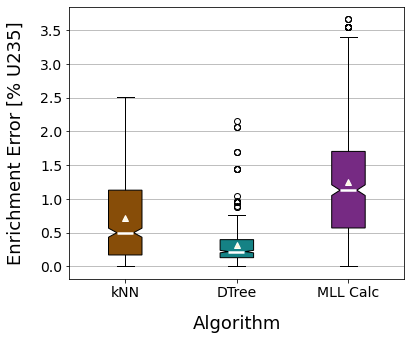
\includegraphics[width=\textwidth]{./chapters/exp1/sfcompo_boxplots_impnull_enri.png}
    \caption{Box plots of enrichment errors using mean-imputed null values.}
    \label{fig:enriimp}
  \end{subfigure}
  \hfill
  \begin{subfigure}[b]{0.49\textwidth}
    \centering
    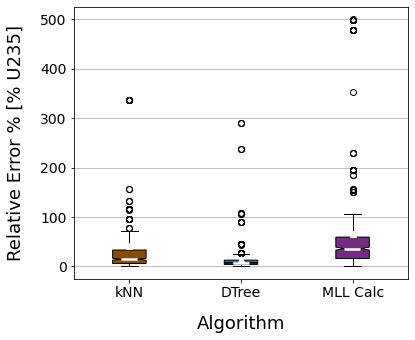
\includegraphics[width=\textwidth]{./chapters/exp1/sfcompo_boxplots_impnull_pcterr_enri.png}
    \caption{Box plots of enrichment percentage errors using mean-imputed null values.}
    \label{fig:enriimppct}
  \end{subfigure}
  \vskip\baselineskip
  \begin{subfigure}[b]{0.49\textwidth}
    \centering
    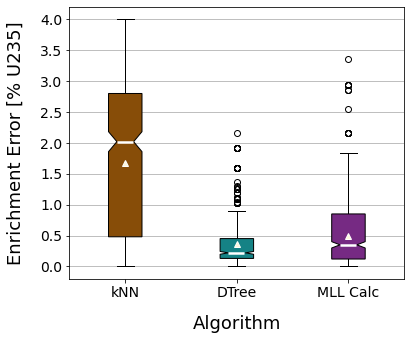
\includegraphics[width=\textwidth]{./chapters/exp1/sfcompo_boxplots_0null_enri.png}
    \caption{Box plots of enrichment errors using zero-replaced null values.}
    \label{fig:enri0}
  \end{subfigure}
  \hfill
  \begin{subfigure}[b]{0.49\textwidth}
    \centering
    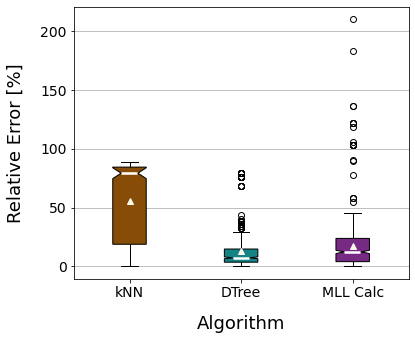
\includegraphics[width=\textwidth]{./chapters/exp1/sfcompo_boxplots_0null_pcterr_enri.png}
    \caption{Box plots of enrichment percentage errors using zero-replaced null values.}
    \label{fig:enri0pct}
  \end{subfigure}
  \caption{Box plots of enrichment prediction errors and percentage errors for 
           each algorithm using two missing entry techniques: imputation with 
           mean values and replacement with zero.}
  \label{fig:sfcoenri}
\end{figure}

Again, a look at the relative errors gives a different sense of these results.
Figures \ref{fig:enriimppct} and \ref{fig:enri0pct} present the percent error
statistics for the imputed nulls and zero-nulls test sets, respectively.  In
Figure \ref{fig:enriimppct} there are 57, 39, and 49 outliers for the
\textit{k}-nearest neighbors, decision trees, and \gls{MLL} calculations,
respectively.  In Figure \ref{fig:enri0pct} there are 44 and 23 outliers for
the decision trees and \gls{MLL} calculations, respectively.

As with the burnup regression, the high percentage errors are caused by a large
overprediction of enrichments that are of low value. All of the \gls{PHWR}s fit
into this category, and removing them from the results removes the outliers
with the highest errors from the imputed nulls results in Figure
\ref{fig:enriimppct}, leaving a maximum of 250\% enrichment error. This is
still a high maximum error because there are other low enrichments not
belonging to the \gls{PHWR} class that remain overpredicted.  As with the
burnup, removing \gls{PHWR}s does not significantly alter the zero-nulls
results in Figure \ref{fig:enri0pct}.

Unlike the case with burnup, the decision trees algorithm gives a better
performance that is null handling-independent than the other algorithm/test set
scenarios. Although there was a slightly worse mean absolute error for the
zero-nulls test set (the median absolute error was the same), the relative
error remains below 100\% for all outliers, as seen in Figure
\ref{fig:enri0pct}.  This makes the decision trees algorithm with the
zero-nulls test set the best performing case for enrichment regression.

It is again true that investigating relative error statistics alongside
absolute error statistics provides a fuller picture of the regression of the
\gls{SFCOMPO} database entries.  It is an unexpected result to have either one
of the scikit algorithms outperform \gls{MLL} calculations for the zero-nulls
test set, since they tended to have lower errors using the imputed nulls test
set. 




\section{Summary}

This chapter covers the details of the methodology in four main sections:
training set simulations, information reduction, statistical methods
implementation, and performance evaluation. This approach focuses on the
situation where there are only nuclides present in the training sets that 
are measured in a non-destructive manner, i.e., via gamma detectors. 

First, in Section \ref{sec:training2}, the training data is simulated using the
same inputs as in Section \ref{sec:training1}. For this training set, however,
the features tracked are 32 radionuclides.

%Second, in Section \ref{sec:inforeduc2}, information reduction on the training
%set is carried out using computationally generated gamma spectra.  The training
%set is initially comprised of nuclide activities, and \gls{GADRAS} is used to
%compute the gamma spectra via \gls{DRF}s for six detectors \cite{gadras} using
%the inputs of the nuclide activity measurements for each \gls{SNF} entry.
%Next, each detector-based training set undergoes three different methods of
%processing the gamma spectra. First, an automatic peak search determines which
%peaks will be tracked, which is different for each detector. Second, a list of
%target gamma energies is created using an arbitrary intensity threshold, so
%that the most likely to be detected gamma energies are tracked. Third, the
%intensity threshold is increased so that the gamma energies list will both be
%shorter and more likely to result in photopeaks at those locations.  The target
%gamma energies are then found on each spectrum, then the counts over a window
%are summed (the window size is determined by detector energy resolution). The
%three lists are thus denoted as the auto, short, and long energy windows lists
%in the upcoming discussion.  These training sets are intended to answer the
%question of whether field-deployable detectors can give enough information
%about radionuclides to be able to successfully attribute \gls{SNF}. 

Second, in Section \ref{sec:inforeduc2}, information reduction on the training
set is carried out using computationally generated gamma spectra.  The training
set is initially comprised of nuclide activities, and \gls{GADRAS} computes the
gamma spectra via \gls{DRF}s for six detectors \cite{gadras} using the inputs
of the nuclide activity measurements for each \gls{SNF} entry.  Each
detector-based training set undergoes processing by summing the counts of the
bins of each energy window from three different lists: the auto, short, and
long energy windows lists.  These training sets are intended to answer the
question of whether field-deployable detectors can give enough information
about radionuclides to successfully attribute \gls{SNF}. 

Third, in Section \ref{sec:statmodel2}, the updates to the algorithm
implementation from Section \ref{sec:statmodel1} are covered. The three
algorithms, \textit{k}-nearest neighbors, decision trees, and \gls{MLL}
calculations, are used to train models to predict the four reactor parameters
of interest. The new training sets also first underwent hyperparameter
optimization.

Fourth, in Section \ref{sec:eval2}, the prediction errors are presented to
evaluate the ability of this methodology to attribute \gls{SNF} with
non-destructive measurements of radionuclides. The reactor type classification
is discussed in Section \ref{sec:exp2_rxtr} and the regression cases are
discussed in Section \ref{sec:exp2_reg}.  The performance of the prediction of
reactor parameters is measured by using test cases drawn from the training set.

The reactor type classification results are presented in Section
\ref{sec:exp2_rxtr}.  The \gls{MLL} calculations consistently perform the best
across the algorithms, and the short energy windows list has the best
performance across the energy windows lists.  Most of the misclassifications
are \gls{PWR} and \gls{PHWR} being labeled as \gls{BWR}.  The automatic peak
searching results in erratic behavior for the scikit-learn algorithms because
the high energy resolution detectors perform poorly but one of the lower energy
resolution detectors performed very well. Most of the algorithm-detector
combinations do not exceed the baseline, and the only cases that do are the
\gls{MLL} calculations for the lab-based \gls{HPGe} with all three energy
windows lists and the \gls{MLL} calculations for the \gls{SrI2} detector with
the auto energy windows list. \textit{Since most of the detector-based data
points do not exceed the baseline for balanced accuracy, reactor type
classification only meets the standard defined using mass-based information for
the four aforementioned cases and the three full-knowledge training sets.}

Next, the regression cases are shown in Section \ref{sec:exp2_reg}.  The burnup
predictions for all the algorithms and energy windows lists outperform the
baseline, except in one case of \textit{k}-nearest neighbors being used with
the auto energy windows list.  The enrichment predictions for the set of six
detectors all falls below the baseline, however, and the time since irradiation
predictions all are very close to the baseline, with some points right above it
and some right below it.  The spread of outliers encompasses $3-17\%$ of the
training set depending on the case, and in most cases the magnitude of the
outlier errors is of significant concern, although most of the median errors
paint a better picture of the performance.  \textit{Based on the performances
relative to the baseline for each regression case, burnup performs above the
standard, enrichment performs far under the standard, and time since
irradiation has several cases that perform on or near the baseline and thus are
very close to the minimum standard.}

For all three regression cases, there is little contrast among the three energy
windows lists. The auto list has more erratic behavior, and the short list has
a slight but not significant average performance over the long list.
\textit{This indicates that the performance of the methodology in this work is
independent of the gamma spectra processing approaches.}

